\documentclass[12pt,a4paper,oneside]{book}
\usepackage[utf8]{inputenc}
\usepackage[spanish]{babel}
\usepackage{amsmath}
\usepackage{amsfonts}
\usepackage{amssymb}
\usepackage{latexsym}
\usepackage{makeidx}
\usepackage{graphicx}
\usepackage{graphics}
\usepackage{lmodern}
\usepackage{hyperref}
\usepackage{subcaption}
\usepackage{pgfplots}
\usepackage{dsfont}
\usepackage{multicol}
\usepackage{xcolor}
\usepackage{booktabs}
\usepackage{float}
\usepackage{subcaption}
\usepackage{wrapfig}

\pagestyle{myheadings}\markboth{Daniel Vázquez Lago}{Daniel Vázquez Lago}

\pgfplotsset{width=10cm,compat=1.9}
\usepgfplotslibrary{external}


\setlength{\parindent}{0px}
\usepackage[left=2cm,right=2cm,top=4cm,bottom=2cm]{geometry}

\author{Daniel Vázquez Lago}
\title{Apuntes Termodinámica II}

\begin{document}

\newcommand{\parentesis}[1]{\left( #1  \right)}
\newcommand{\parciales}[2]{\frac{\partial #1}{\partial #2}}
\newcommand{\pparciales}[2]{\parentesis{\parciales{#1}{#2}}}
\newcommand{\D}{\mathrm{d}}
\newcommand{\corchetes}[1]{\left{ #1  \right} }
\newcommand{\ccorchetes}[1]{\left[ #1  \right]}
\newcommand{\cte}{\mathrm{cte}}
\newcommand{\tquad}{\quad \quad \quad}
\newcommand{\Jn}{\textbf{J}}
\newcommand{\Fn}{\textbf{F}}
\newcommand{\Omegan}{\mathbf{\Omega}}
\newcommand{\divergencia}{\nabla \cdot}
\newcommand{\rotacional}{\nabla \times}
\renewcommand{\div}{\nabla \cdot}
\newcommand{\logn}{\mathrm{ln} \ }
\newcommand{\rot}{\nabla \times}
\newcommand{\grad}{\nabla }
\newcommand{\inti}{\int_{-\infty}^{\infty}}
\newcommand{\into}{\int_{0}^{\infty}}
\newcommand{\muJK}{\mu_{JK}}


\maketitle

\newpage

\tableofcontents

\newpage

\chapter{Gases ideales}

\section{Ecuación térmica del cas ideal}


La ecuación térmica de un sistema en equilibrio termodinámica se representa por:

\begin{equation}
X_i = X_i (T,x_k,n_j)
\end{equation}

donde $n_j$ son las componentes (variables de composición) y $X_i$ son las fuerzas generalizadas asociadas a una variable de deformación $x_i$. T es la temperatura absoluta del sistema. Para un gas monocomponente y en un sistema cerrado la ecuación térmica del sistema en equilibrio será:

\begin{equation}
p = p(T,v)
\end{equation}

donde $v=V/n$. Si se representa gráficamente el cociente $pv/T$ frente a la presión $p$ a una temperatura dada constante obtenemos curvas en el plano, representación que se llama \textit{diagrama de Amagat}. El comportamiento de cada gas es diferente para cada temperatura, sin embargo si se extrapola el comportamiento cuando $p \rightarrow 0$ todas las curvas (isotermas) tienden al mismo valor. Este valor es conocido como la \textit{constante universal de los gases} y se representa por $R$, definida como:

\begin{equation}
R = \lim_{p \rightarrow 0} \parentesis{\dfrac{pv}{T}}
\end{equation}

Definimos como \textbf{gas ideal} a un gas hipotético que verifica no solo que si $p \rightarrow 0 $ dicho cociente tiende a $R$, si no que para \textit{cualquier} presión dicho cociente es $R$.  Entonces se verificará lo que conocemos como \textbf{ecuación térmica de estado del gas ideal} o la \textbf{ecuación de Clapeyron}:

\begin{equation}
pV = nRT
\end{equation}

\section{Ecuación energética}

Como sabemos la termodinámica es una ciencia empírica: trata de modelizar y darle una explicación a fenómenos experimentales. Algunas veces lo hace mejor que otras, y cuanto mas sencillo sea el modelo mas distancia con la realidad habrá. Sin embargo muchas veces sirve como primera aproximación a la realidad. La deducción de la ecuación energética del gas ideal no iba a ser una excepción, y para entender como se deduce tendremos que hablar antes de la experiencia de Joule. \\

Joule estudio como se comportaba la energía interna de un gas. En líneas generales fue capaz de demostrar (aunque muchas de ellas debidas a las limitaciones tecnológicas de la época) que la variación de energía interna de un gas no dependía del volumen del gas. Para esto diseño un experimento en el cual un gas se expandía en el vacío (no hay trabajo mecánico) y que no intercambiaba calor con el medio (sumergía dicho gas en un líquido, y al no variar la temperatura del mismo dedujo que no hubo intercambio calorífico). Es decir el \textit{coeficiente Joule} definido como:

\begin{equation}
\mu_J = \pparciales{T}{V}_U
\end{equation}

es cero. Esto le llevo a definir la que hoy conocemos como \textbf{ley de Joule}: \textit{la energía interna de un gas depende exclusivamente de la temperatura}. De otra forma:

\begin{equation}
U = U(T)
\end{equation}

que como consecuencia de ello se puede escribir la \textit{forma diferencial de la ecuación energética} del gas:

\begin{equation}
\D U = C_V \D T = n c_V \D T
\end{equation}

En experimentos mas actuales se ha demostrado que $U=U(T,p)$. 

\section{Gas perfecto}

Definimos como \textbf{gas perfecto} a aquel gas que cumpliendo lo mismo que un gas ideal (ecuación de clapeyron, energía interna función de temperatura...) verifica además que $C_V$ es una constante, y no depende de la temperatura. En ese caso podremos integrar la forma diferencial llegando a:

\begin{equation}
\Delta U = C_V \Delta T = n c_V \Delta T
\end{equation}

Para un gas perfecto la \textit{ley de Mayer} tal que:

\begin{equation}
C_X - C_x = \dfrac{T \alpha^2 x}{k_T} 
\end{equation}

se reduce a:

\begin{equation}
C_p - C_V = nR
\end{equation}

que es la llamada \textit{forma analítica de la ley de Mayer para un gas ideal}. Puede demostrarse que para un gas perfecto la entalpía viene dada por:

\begin{equation}
\Delta H = C_p \Delta T
\end{equation}

y que la entropía por:

\begin{equation}
S = n (c_p \log (T) - R \log (p) + s_0)
\end{equation}

\section{Trasformaciones adiabáticas de un gas perfecto}

Las transformaciones adiabáticas de un gas perfecto o ideal cobran mucha importancia a la hora de resolver problemas y ejercicios, por ello traemos aquí como se deducen las relaciones de $p$, $V$ y $T$ entre ellas si no se intercambia calor con el entorno. Para esto es fundamental definir un parámetro: el \textit{coeficiente adiabático} $\gamma$. Este parámetro se define como

 \begin{equation}
\gamma = \frac{c_p}{c_v}
\end{equation}

Ahora sí, comencemos. Tenemos que por definición $\D U = \D W$ si $\D Q = 0$. Desarrollando esto llegamos a que:

$$
n c_V \D T = - p \D V \rightarrow n c_V \D T = - \dfrac{nRT}{V} \D V \rightarrow \dfrac{c_v}{R} \dfrac{\D T}{T} = - \dfrac{\D V}{V}
$$

ahora desarrollando $R=c_p - c_v $, pasando el $c_V$ como cociente llegamos a que:

\begin{equation}
\dfrac{1}{\gamma -1} \dfrac{\D T}{T} = \dfrac{\D V}{V}
\end{equation}


que si integramos para un gas perfecto donde $C_V$ y $C_p$ son constantes tenemos que:

\begin{equation}
T_i V_i^{\gamma-1} = T_f V_f^{\gamma-1} 
\end{equation}


\begin{equation}
p_i V_i^{\gamma} = p_f V_f^{\gamma}
\end{equation}


\begin{equation}
p_i^{1-\gamma} T_i^{\gamma} = p_f^{1-\gamma} T_f^{\gamma} 
\end{equation}


\section{Transformaciones politrópicas}

Para un proceso cualquiera que sufra un sistema hemos definido la capacidad calorífica mediante la relación:

\begin{equation}
C_a = \parentesis{\dfrac{\D Q}{\D T} }_a
\end{equation}

Se denomina \textbf{transformación politrópica} a aquella en la que a capacidad calorífica del sistema $C_a$ permanece constante durante el proceso. Ejemplos de ellos son $C_p$ y $C_V$, ya que se mantienen constantes en un proceso donde se conserva una cantidad (presión y volumen). Esto es válido para cualquier gas, real o ideal: si un proceso es politrópico $C_a$ permanece constante. \\

En el caso de que estemos hablando de un gas ideal, como $\D U = C_V \D T$ tenemos que:

$$ C_V \D T = C_a \D T - \dfrac{nRT}{V} \D V \rightarrow  \dfrac{\D T }{T} + \dfrac{C_p - C_V}{C_V - C_a} \dfrac{\D V}{V} = 0 $$


entonces si definimos el \textbf{índice de politropía} $n$ como:

\begin{equation}
n = \dfrac{C_p - C_a}{C_V - C_a} ; \tquad n -1 = \dfrac{C_p - C_V}{C_V - C_a}
\end{equation}


tenemos que la anterior relación se puede escribir como:

\begin{equation}
\dfrac{\D T}{T} + (n-1) \dfrac{\D V}{V} = 0
\end{equation}

que nos lleva, si integramos, a:



\begin{equation}
T_i V_i^{n-1} = T_f V_f^{n-1} 
\end{equation}


\begin{equation}
p_i V_i^{n} = p_f V_f^{n}
\end{equation}


\begin{equation}
p_i^{1-n} T_i^{n} = p_f^{1-n} T_f^{n} 
\end{equation}

Teniendo en cuenta el concepto de transformación politrópica se pueden deducir fácilmente que las transformaciones isócora (n=$\infty$), isóbara (n=0), isoterma (n=1), adiabática (n = $\gamma$) son casos particulas de las transformaciones politrópicas.


\section{Mezcla gases perfectos}

\subsection{Presiones parciales}

Definimos como \textbf{mezcla ideal de gases perfectos} a aquella mezcla que verifica la ecuación térmica de estado de gas ideal. Si $n$ son los moles totales de la mezcla (los moles de todos los diferentes gases sumados), $p$ la presión de la mezcla y $T$ su temperatura debe verificarse que:

\begin{equation}
p = n \dfrac{RT}{V} = \parentesis{\sum_i n_i} \dfrac{RT}{V} = \sum \parentesis{ n_i \dfrac{RT}{V}}
\end{equation}

Además debe verificarse que su energía interna a una temperatura dada es la suma de la que tendrían los gases que la constituyen, en un estado puro y a la misma temperatura que la mezcla:

\begin{equation}
U = \sum_i U_i^0 = \sum_i n_I u_i^0
\end{equation}

La \textbf{ley de Dalton} o \textbf{ley de las presiones parciales} es una ley experimental (que como la experiencia de Joule fue afectada por las carencias tecnológicas) que nos dicen que la suma de las presiones que ejercen por separado una mezcla de gases en un recipiente es igual a la presión ejercida al introducir todos los gases a la vez (a la misma temperatura). \\

Si definimos como \textbf{presión parcial} $p_i$ como la presión que ejercería el gas $i$ si él sólo ocupase el volumen total de la mezcla con la misma temperatura la ley de Dalton nos lleva a que:

\begin{equation}
p_i = \chi_i \cdot p
\end{equation}

donde $p$ es la presión total de la mezcla y $\chi_i$ es la \textit{fracción molar} tal que:

\begin{equation}
\chi_i = \frac{n_i}{n}
\end{equation}

\subsection{Teorema de Gibbs}

El \textbf{teorema de Gibbs} establece que \textit{la entropía de una mezcla de gases perfectos no reaccionantes es siempre igual a la suma de las entropías parciales}. Si definimos \textbf{entropía parcial} como la entropía que tendría dicho gas si ocupase él solo el volumen de la mezcla y a la misma temperatura que esta. \\

El teorema de Gibbs es también válido para cualquier potencial termodinámico. 

\chapter{Gases reales}

\section{Coordenadas críticas}

Todos los gases se comportan como ideales a bajas presiones y temperaturas altas. Cuanto mas nos separemos de estas condiciones un comportamiento cada vez mas complicado surgirá. Cuando tratamos de estudiar el comportamiento de un gas real alejado de dichas condiciones sus ecuaciones fundamentales se vuelven analíticamente complicadas, por lo que es mas conveniente analizar sus propiedades en términos de ecuaciones de estado.\\

Comencemos definiendo el \textbf{factor de compresibilidad} $z$ (molar) como el cociente entre el volumen real para un gas a $T$ y $p$ dadas y el mismo volumen de un gas ideal en dichas condiciones:

\begin{equation}
z = \dfrac{v_{real}}{v_{ideal}} = \dfrac{p v_{real}}{RT}
\end{equation}


\begin{figure}[h!]
    \centering
    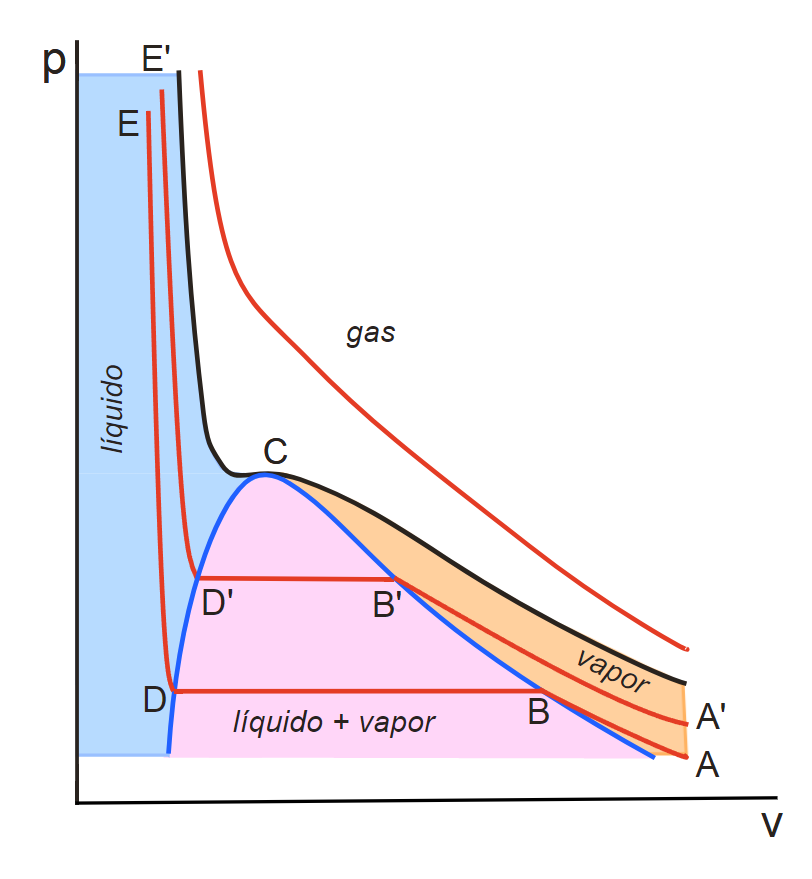
\includegraphics[width=0.39\textwidth]{isotermas-andrews.png}
    \caption{Isotermas de Andrews}
\end{figure}


Si continuamos estudiando el comportamiento de un gas real, y representamos en  un diagrama $p-v$ un conjunto de isotermas correspondientes para un gas dado. Para algunas de las isotermas el gas pasará, a medida que aumentemos o disminuyamos el volumen, de una fase líquida, a una fase gaseosa o un equilibrio entre ambas. Extendemos las isotermas aún en las zonas donde se produce la condensación. A estas isotermas las llamaremos \textit{isotermas de Andrews}. \\


Denominamos como \textbf{temperatura crítica} a la temperatura para la cual una temperatura mayor no permite condensar al gas mediante una compresión isoterma. La curva negra en la imagen representa la isoterma para la temperatura crítica (\textit{isoterma crítica}).\\


 Al punto de inflexión $C$ de dicha isoterma es conocido como \textbf{punto crítico} y sus coordenadas $p_c,v_c,T_c$ son las \textit{coordenadas críticas} Si pasamos trazamos una curva divide las regiones líquido-vapor (es decir, la curva que diferencia el sistema con una fase al sistema con dos fases) tenemos la \textbf{curva de saturación}. \\

Para una representación del producto $p \cdot v$ frente a $p$ para isotermas obtenemos lo que se llama el \textit{diagrama de Boyle}. Si representamos las isotermas podremos ver que a en cierto rango de las temperaturas las isotermas presentan un mínimo. La curva que une todos estos mínimos se la conoce como \textbf{curva de Boyle}, y representa los puntos para los cuales $k_T^{ideal} = k_T$. \\
 
Esto es porque:

$$ \pparciales{(pv)}{p}_T  = v + p \pparciales{v}{p}_T = pv \ccorchetes{\dfrac{1}{p} + \dfrac{1}{v} \pparciales{v}{p}_T} $$

y como $$k_T^{ideal}=1/p$$ $$k_T = - \frac{1}{v} \pparciales{v}{p}_T$$ tenemos que:

\begin{equation}
\pparciales{(pv)}{p}_T   = pv(k_T^{ideal} - k_T)
\end{equation}

por lo que si estamos en un mínimo, dicha derivada parcial será cero y los coeficientes de compresibilidad se igualarán. La temperatura máxima para la cual obtenemos un mínimo se conoce como \textbf{temperatura de Boyle}. El punto de intersección con la isoterma de la temperatura de Boyle con el eje de ordenadas se conoce como \textbf{punto de Boyle}. Esta temperatura también se define como:

\begin{equation}
\lim_{p \rightarrow 0} \pparciales{(pv)}{p}_{T_B} = 0
\end{equation}

El significado físico de esta curva es muy importante (si no no lo mencionaríamos). En aquella zona donde las pendientes sean negativas (izquierda de la curva de Boyle) tenemos que el gas real es mas comprensible que el gas ideal, y para aquella zona donde sean positivas el gas ideal es mas compresible que el gas real.

\section{Estrangulación adiabática. Coeficiente de Joule-Kelvin}

Experimentalmente si un gas o líquido fluyen y de se encuentran con un obstáculo que provoca un estrechamiento, y luego vuelve a expandirse, la presión del fluido tras expandirse es menor que la presión antes de la estrangulación. Si esta \textit{estrangulación} es \textit{adiabática}, al efecto que se produce en dicha expansión sobre el gas se le denomina \textit{efecto Joule-Thomson}. \\

Experimentalmente se tiene que en un experimento de Joule-Thomson al ser adiabático $\D Q=0$ debe verificarse (si fuera un proceso reversible) que:

\begin{equation}
U(T_1,p_1) + p_1 V_1 = U(T_2,p_2) + p_2 V_2
\end{equation}

es decir que:

\begin{equation}
H_1 = H_2
\end{equation}

pero es importante recordar esto: la isoentálpica \textit{no} es la línea que representa el proceso de estrangulación adiabática sino que es la curva que representa un proceso \textit{reversible} entre los mismos estados entre los que tiene lugar el proceso \textit{irreversible} de estrangulación adiabática. \\

Experimentalmente la expansión de Joule-Thomson para gases reales, en función del a presión y temperatura inicial, genera fenómenos diferentes. Si la temperatura inicial es una temperatura elevada, los gases se calentarán; si la temperatura es baja y una presión no muy elevada, los gases se enfriarán. Por lo tanto tiene que haber una temperatura para la cual cambia de signo la variación de la temperatura por este efecto. A dicha temperatura se la conoce como \textbf{temperatura de inversión}.\\

Para estudiar el comportamiento del gas lo que hacemos es un diagrama T-p del gas, seleccionando desde un estado de equilibrio ($T_1,p_1$) una presión final de valor $p_2$ y midiendo su temperatura $T_2$. Representando esto obtenemos un conjunto de isoentálpicas:

\begin{figure}[h!] \centering
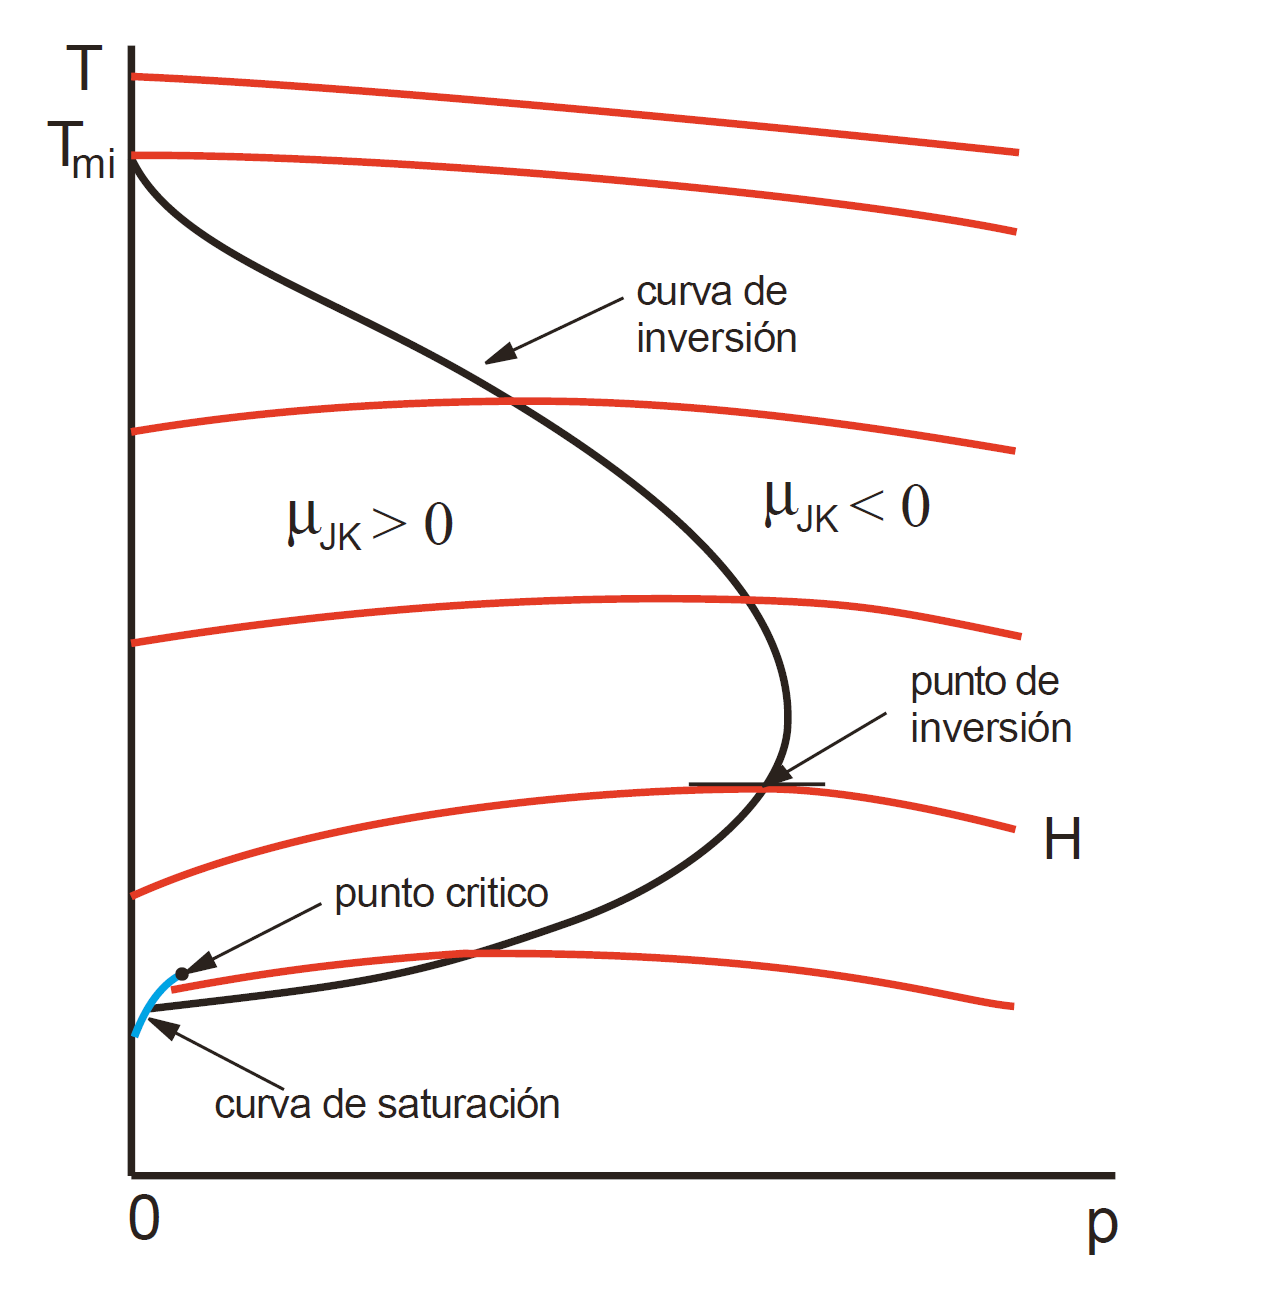
\includegraphics[scale=0.3]{isoentalpicas.png}
\caption{curva de inversión}
\end{figure}


Definimos como el \textbf{coeficiente de Joule-Kelvin} $\mu_{JK}$ o $\mu_{JT}$ a:
\begin{equation}
\mu_{JK} = \pparciales{T}{p}_H
\end{equation}


Los puntos de inversión son los que verifican que $\muJK = 0$. Así pues este coeficiente nos da una medida de como se comportan los gases tras el efecto Joule-Thomson. A la izquierda de la curva el coeficiente será positivo y por lo tanto en la expansión ($\Delta p <0$) el gas se enfriará, y a la derecha de la curva será positivo y por lo tanto en la expansión ($\Delta p < 0$) se calentará. \\

Describir este coeficiente de manera analítica respecto otros coeficientes puede ser bastante tedioso. Sin embargo en general se puede calcular de la siguiente forma:

$$ \pparciales{T}{p}_H \pparciales{p}{H}_T \pparciales{H}{T}_p=-1; \quad \pparciales{H}{T}_p =C_p; \quad \D H = T \D S + V \D p; \quad \D S = \dfrac{C_p}{T} \D T - \pparciales{V}{T}_p \D p $$

Esto todo implica que:

\begin{equation}
\pparciales{T}{p}_H = - \dfrac{1}{C_p}  \ccorchetes{V-T\pparciales{V}{T}_p} = \dfrac{V}{C_p} (T \alpha -1)
\end{equation}

\section{Ecuaciones térmicas de estado}

\subsection{Van der Waals}

La ecuación de estado de Van der Waals es un desarrollo puramente teórico que a partir de la ecuación de Clapeyron crea una nueva ecuación térmica de estado, añadiendo ciertos términos que predice mejor el comportamiento de los gases reales, tales como la condensación y otros fenómenos. Vamos a tratar primero de mencionar cuales son los pasos y conceptos que desarrollo Van der Waals para llegar a su ecuación de estado. \\

En primer lugar el consideró que cuando escribimos $V$ en la ecuación realmente no estamos escribiendo todo el volumen que tiene disponible el sistema para moverse, ya que hay cierto volumen que es ocupado por las moléculas. Entonces tendríamos que restarle al volumen $V$ del recipiente un factor $bn$ donde $b$ es el volumen que ocupa cada molécula y $n$ el número de moléculas. Entonces el volumen real disponible para el movimiento de un gas sería $V-nb$. \\
 
El segundo factor que desarrolló tiene que ver con la presión. La existencia de fuerzas intermoleculares es algo que no se tiene en cuenta a la hora de desarrollar la teoría cinética de los gases ideales, y sin embargo tienen mucha importancia. Consideremos una pared. Está claro que una molécula cerca de la pared solo tiene moléculas debajo. Si existiese una fuerza intermolecular atractiva entre las moléculas, está claro que cualquier molécula cerca de la pared sufriría una fuerza que ralentizase su movimiento hacia la pared y por tanto la presión que medimos sería menor que en el centro de la masa gaseosa, donde debido a que hay moléculas en todas partes la fuerza neta sería nula. Consecuentemente Van der Waals dijo que la presión que somos capaces de medir es menor que la presión real del gas. Si el coeficiente $a$ es una medida de cuanta fuerza intermolecular hay, tenemos que el término que debemos añadir será $a(n/V)^2$. Ahora bien, ¿Por qué $(N/V)^2$? Pues porque la cantidad de fuerza intermolecular será proporcional a la densidad de moléculas (cuanta mas densidad haya mas fuerte se tirará para atrás de nuestra molécula), y al cuadrado porque el número de choques con la pared también depende de la densidad molecular. \\

Por tanto nuestra nueva ecuación será:

\begin{equation}
\ccorchetes{p+a\parentesis{\dfrac{n}{V}}^2} (V-bn) = nRT
\end{equation}

y si la dividimos entre $n$ tendremos la forma mas conocida, llamada la \textbf{ecuación de Van der Waals}:

\begin{equation}
\ccorchetes{p+\dfrac{a}{v^2}} (v-b) = RT
\end{equation}

Si desarrollamos nuestra función de forma que:

\begin{equation}
pv^3 - (pb+RT)v^2 +a v - ab = 0
\end{equation}

Tenemos que en función de la temperatura, la curva para cada isoterma tendrá diferentes soluciones. Cuando la temperatura hace que las 3 raíces sean iguales entre sí (y reales), se anularán en un punto denominado el punto crítico tal que sus coordenadas son ($p_c,v_c,T_c$). Este punto además se verificará que:

\begin{equation}
\pparciales{p}{v}_{T_c} = 0, \tquad \pparciales{^2 p}{v^2}_{T_C} = 0
\end{equation}

A estas coordenadas las llamamos \textbf{coordenadas críticas}, y podemos despejar $a,b,R$ en función de estas. Se puede comprobar que para un gas de Van der Waals se verifica que:

\begin{equation}
U = U(T,V)
\end{equation}

y que $C_V \neq C_V(V)$.

\subsection{Ecuación del virial}

Las ecuaciones del virial no son mas que el desarrollo de potencias del producto de $pv$, bien de la presión o de la inversa del volumen molar:

\begin{equation}
pv = A + B \dfrac{1}{v} + C \parentesis{\dfrac{1}{v}}^2 + \cdots = A + \dfrac{B}{v} + \dfrac{C}{v^2} + \cdots 
\end{equation}

o bien de la presión:

\begin{equation}
pv = A' + B' p + C' p^2 + \cdots
\end{equation}

En estas ecuaciones $A,B,C...$ y $A',B',C'...$ se llaman \textit{coeficientes del virial} y se pueden relacionar entre sí. Además dado que se debe verificar que:

\begin{equation}
\lim_{p \rightarrow 0} \parentesis{\dfrac{pv}{T}} = R
\end{equation}

por lo que $A' = RT$, y como $A=A'$ tenemos que $A=RT$. Entonces:

\begin{equation}
\dfrac{pv}{RT}  = 1 + \dfrac{B}{RT v} + \dfrac{C}{RT v^2} + \cdots = 1 + \dfrac{B' p}{RT} + \dfrac{C' p^2}{RT} + \cdots
\end{equation}

lo que nos revela que los diversos coeficientes del virial representan simplemente correcciones respecto al comportamiento ideal.


\section{Diagrama de comprensibilidad generalizado}

Las ecuaciones de estado de los gases reales que hemos analizado y se van a presentar en esta asignatura vienen dadas de la forma:

\begin{equation}
f(p,v,T,a,b,...) = 0
\end{equation}

donde estos $a,b,...$ son parámetros característicos de cada gas. Para la mayoría de ecuaciones podemos substituirlos por las coordenadas críticas:

\begin{equation}
f(p,v,T,p_C,v_C,T_C...) = 0
\end{equation}

Si el comportamiento de $p_C,T_C,v_C$ es lineal (si aparecen otras potencias o funciones analíticas) podemos crear unas nuevas variables denominadas \textbf{variables de estado reducidas} definidas mediante:

\begin{equation}
p_r = \dfrac{p}{p_C} \tquad v_r = \dfrac{v}{v_C} \tquad T_r = \dfrac{T}{T_C}
\end{equation}

tal que la función queda de manera que:

\begin{equation}
f(p_r,v_r,T_r) = 0
\end{equation}

Esta es la denominada \textbf{ecuación de estado reducida}. Es única para todos los gases que obedezcan la misma ecuación térmica de estado. En general solo es válida para ecuaciones con 2 parámetros característicos ya que con mas se perdería la linealidad anteriormente citada. Entonces esto nos revela una ley muy potente: la \textbf{ley de los estados correspondientes}: si cantidades equimoleculares de dos fases cualquiera, cuyo comportamiento se puede expresar mediante la misma ecuación de estado reducida, tales que dos coordenadas reducidas son iguales, tenemos que necesariamente la tercera coordenada será igual. En este caso decimos que los gases se encuentran en \textit{estados correspondientes}. \\

Si representamos en un diagrama z-p los comportamientos de diferentes gases tenemos que las isotermas difieren entre ellos. Sin embargo la ley de estados correspondientes nos permite desarrollar un diagrama de comprensibilidad generalizado que es aplicable en buena aproximación a todos los gases. A este diagrama se le llama \textbf{diagrama de compresibilidad generalizado} tal que:

\begin{equation}
z = \dfrac{p_C v_C}{R T_C} \dfrac{p_r v_r}{T_r} = z_C \dfrac{p_r v_r}{T_r} = C \dfrac{p_r v_r}{T_r}
\end{equation}

donde $C$ es una constante universal obtenida del promedio de los valores de $z_C$ de una gran muestra de gases. A partir de estas curvas es posible deducir el valor tanto de la presión, como del volumen, o de la temperatura de cualquier gas si se conocen las otras dos variables.



\chapter{Transiciones de fase}

\section{Condiciones de equilibrio para sistemas heterogéneos}

Definimos \textbf{fase} como cada una de las partes del sistema que tiene en todo punto la misma composición química e idénticas propiedades físicas características (densidad, índice de refracción, conductividad...). Así pues las distintas fases de un sistema pueden ser separadas entre sí por medios físicos.\\

Vamos a establecer qué condiciones se deben verificar par que un sistema heterogéneo y multicomponente tenga sus distintas fases en equilibrio, i.e. esté en \textit{equilibrio de fases}. \\

Consideremos un sistema cerrado constituido por $c$ componentes inertes entre sí y $F$ fases, con el volumen como única \textit{variable extrínseca}. Analizando la energía interna de cada fase $(\alpha)$:

$$ \D U^{(\alpha)} = T^{(\alpha)} \D S^{(\alpha)} + p^{(\alpha)} \D V^{(\alpha)} + \sum_{i=1}^c \mu_i^{(\alpha)} \D n_i^{(\alpha)} $$

y para un sistema en su conjunto tenemos que:

$$  U^{(\alpha)} = \sum_{\alpha=1}^F  \parentesis{T^{(\alpha)} \D S^{(\alpha)} + p^{(\alpha)} \D V^{(\alpha)} + \sum_{i=1}^c \mu_i^{(\alpha)} \D n_i^{(\alpha)}} $$

Para un sistema en equilibrio el \textit{principio de mínima energía} exige que sea nula todos los desplazamientos virtuales. Además hemos impuesto al sistema que no sea móvil (el volumen global del sistema se conserva) que sea cerrado (el número de moles de cada substancia se conserva) y que todos los procesos que ocurran en el sean adiabaticamente reversibles (la entropía se conserva).\\

Debido a esto se tiene que verificar que:

\begin{equation}
\D S^{(1)}= - \sum_{\alpha=2}^F \D S^{(\alpha)}; \tquad \D V^{(1)} = - \sum_{\alpha=2}^F V^{(\alpha)}; \tquad \D n_i^{(1)} =- \sum_{\alpha=2}^F \D n_i^{(\alpha)}
\end{equation}


Entonces para que se verifiquen las condiciones de equilibrio se tiene que verificar que:

$$  U^{(\alpha)} = \sum_{\alpha=2}^F  \parentesis{(T^{(\alpha)}-T^{(1)}) \D S^{(\alpha)} + (p^{(\alpha)}-p^{(1)}) \D V^{(\alpha)} + \sum_{i=1}^c (\mu_i^{(\alpha)}-\mu^{(1)}) \D n_i^{(\alpha)}} $$

y por lo tanto para que se mantenga en equilibrio el sistema:

\begin{equation}
\begin{array}{ll}
T^{(1)} = T^{(2)} = & \ldots = T^{(F)} \\
V^{(1)} = V^{(2)} = & \ldots = V^{(F)} \\
\mu_i^{(1)} = \mu_i^{(2)} = & \ldots = \mu_i^{(F)} \\
\end{array}
\end{equation}

Estas son las condiciones generales de equilibrio. Por lo tanto para que todas las fases se encuentren en equilibrio se debe verificar que la temperatura sea  la misma (estén en \textit{equilibrio térmico}), que la presión sea la misma (\textbf{equilibrio mecánico)} y que el potencial químico de cada componente sea el mismo (\textit{equilibrio material}). \\

Por cada ecuación de energía interna de cada fase tenemos una ecuación de Gibbs-Duhem, y así tener $F$ ecuaciones con $c+2$ variables entre sí (que son $\D T, \D p, \D \mu_i$). Es decir tenemos ahora un sistema de ecuaciones, por lo que podemos estudiar en que casos el sistema soluciones algebraicamente. Para que tengamos soluciones propias el número de ecuaciones linealmente independientes debe de s er menor o igual que el número de incógnitas, es decir: $F \leq c+2$. En el caso de ser la igualdad el determinante debe ser cero. \\

En el caso de que $F < c+2$ implica que podemos encontrar $c+2-F$ variables que pueden ser modificadas sin que cambie el número y la naturaleza del sistema (estamos ante un sistema compatible indeterminado). Entonces si llamamos \textbf{grados de libertad} y denotamos por $L$ este a el número de variables intensivas independientes que se pueden modificar sin modificar el equilibrio, llegamos a la \textbf{regla de las fases de Gibbs}:

\begin{equation}
F + L = c +2
\end{equation}


\section{Clasificación de transiciones de fase}

Las transiciones de fase tienen lugar de tal forma que las presiones de las distintas fases son igual es entre sí, lo mismo con la temperatura y los potenciales químicos. Sin embargo otras magnitudes térmicas y caloríficas pueden variar, de manera continua o discontinua, finita o infinita. En base a eso vamos a plantear la clasificación de Ehrenfest de las transiciones de fase.  \\

Para ello recordamos las primeras derivadas del potencial de Gibbs:

\begin{equation}
v = \pparciales{g}{p}_T \tquad s = - \pparciales{g}{T}_p
\end{equation}


y las segundas derivadas:

\begin{equation}
\dfrac{c_p}{T} = \pparciales{s}{T}_p = - \pparciales{^2 g}{T};  \tquad k_T = - \dfrac{1}{v} \parciales{v}{p} = \dfrac{1}{v} \pparciales{^2 g}{p^2};
\end{equation}

\begin{equation}
\alpha = \dfrac{1}{v} \pparciales{v}{T}_p = \dfrac{1}{v} \ccorchetes{\pparciales{}{T} \pparciales{g}{p}}
\end{equation}

Se denomina \textbf{transición de fase de primer orden} a aquellas que presentan una discontinuidad \textit{finita}  en las primeras derivadas del potencial de Gibbs (y en las de segundo orden). En este tipo de transiciones la entropía y el volumen sufren una variación discontinua, por lo que van acompañadas de manifestaciones energéticas en forma de calor y de trabajo. \\

Las \textbf{transiciones de fase de segundo orden} son aquellas que tienen las derivadas de primer orden del potencial de Gibbs continuas y presentan una discontinuidad \textit{finita} en todas o algunas derivadas de segundo orden de dicho potencial. No van acompañadas de manifestaciones energéticas.\\

Las \textbf{transiciones lambda} son aquellas que se conservan las primeras derivadas del potencial de Gibbs y tienen un salto infinito las segundas derivadas. Se le llama así por que su forma es parecida a la letra griega.


\section{Transiciones de fase de primer orden: ecuación de Clausius-Clapeyron}

A un cambio de fase donde la presión, temperatura y fracciones molares de las fases permanecen constantes se le llama \textbf{reacción de fase}. Las reacciones de fase son procesos cuasiestáticos. 


\chapter{Sistemas reactivos}

La composición de un sistema puede variar por al existencia de reacciones químicas en el seno del sistema. Una reacción química es aquel proceso en el que una o varias sustancias (reactivos) se trasforman en otras sustancias (productos). Sin embargo el estudio de las reacciones químicas presentan un problema: las reacciones químicas son un proceso de evolución en el trascurso del tiempo, por lo que la termodinámica del equilibrio no puede analizar satisfactoriamente que ocurre en este proceso. Sin embargo la termodinámica del equilibrio si que puede predecir en que estado final se va a encontrar una vez hallamos llegado al \textit{equilibrio químico}. \\

En una reacción química llamamos \textbf{coeficiente estequiométricos} $v_i$ a la relación que hay entre las sustancias cuando se trasforman. Son resultado del principio de la conservación de la masa, ya que el número de átomos no puede variar. Esto se conoce como \textit{ley de Lavosier}. Estos coeficientes son adimensionales y reales, positivos para los productos y negativos para los reactivos. \\

Cuando tenemos un sistema encerrado por sustancias reactivos, lo mas normal es que se produzca una reacción, trasformando parte de las sustancias en otras. Si suponemos que solo existe una posible reacción entre las sustancias (y el sistema es cerrado) tenemos que la cantidad de moles de una sustancia solo podrá variar debido a dicha reacción. Sean $n_i^0$ son los moles iniciales de dicha sustancia, tenemos que los moles de dicha sustancia al cabo de un tiempo serán:

\begin{equation}
n_i = n_i^0 + v_i \xi 
\end{equation}

siendo $\xi$ el \textbf{grado de avance de la reacción}, una medida de en que grado de realización se encuentra dicha reacción. Siempre es positivo, si es negativo significa que los productos se trasforman en reactivos, por lo que debemos cambiar el sentido de la reacción. Tiene unidad de moles. Tenemos además que se debe verificar que:

\begin{equation}
\D n_i = v_i \D \xi
\end{equation}


Esto implica directamente que el grado de avance es independiente de la sustancia elegida, y que esta relacionado con la velocidad de reacción. Además pone de manifiesto que las variaciones del número de moles de cada una de las sustancias no son independientes entre sí, y que con un único parámetro especificas su variación. Además podemos obtener la fracción molar en función del grado de avance:

\begin{equation}
x_i = \dfrac{n_i}{\sum_i n_i} = \dfrac{n_i^0 + v_i \xi }{n^0 + \Delta v \xi}
\end{equation}

De haber $r$ reacciones linealmente independientes tendríamos $r$ grados de avance distintos.

\section{Calor de reacción}

Cuando se produce una reacción las sustancias cambian su naturaleza, por lo que en este se realiza un intercambio de energía con el medio de tal forma que se intercambia o bien trabajo mecánico o calor. Esta energía aparece por la rotura y formación de enlaces, o el cambio de la distribución espacial de los mismos. \\

Se denomina \textbf{calor de reacción} a la cantidad de energía que el sistema ha de ceder o absorber del entorno cuando se verifica una vez completa la reacción. Si $Q<0$ (cede calor) se denomina \textbf{exotérmica} y si $Q>0$ (absorbe calor) se denomina \textbf{endotérmica}. Llamamos \textit{calor de formación} al calor de reacción que sucede en una reacción cuyo único producto es una sustancia y sus reactivos son los elementos de dicha sustancia en su forma mas estable para la misma presión y temperatura que la sustancia. La entalpía de formación de cualquier elemento se considera cero.
 \\

Tenemos que si el suceso ocurre a presión constante el calor intercambiado coincide con la variación de entalpía, y si ocurre a volumen constante coincide con la variación de energía interna (idealmente):

\begin{equation}
Q_P = \Delta H  \tquad Q_V = \Delta U
\end{equation}

\subsubsection*{Calor a presión constante}

Un proceso a presión constante se verifica que:

\begin{equation}
Q_P = H_f - H_i = \overline{\Delta H}
\end{equation}

si al principio de la reacción solo hay reactivos y al final solo hay productos podemos deducir que: $H_f = \sum_i^p H_i $  y $H_i = \sum_j^r H_j$. En ese caso se denomina a $\overline{\Delta H}$ como \textbf{entalpía de reacción}. 


\subsubsection*{Calor a volumen constante}

En este caso es exactamente igual con el volumen. Un proceso a volumen constante se verifica que:

\begin{equation}
Q_P = U_f - U_i = \overline{\Delta U}
\end{equation}

si al principio de la reacción solo hay reactivos y al final solo hay productos: $U_f = \sum_i^p U_i $  y $U_i = \sum_j^r U_j$. En ese caso se denomina a $\overline{\Delta U}$ como \textbf{energía interna de reacción}. \\



Para ambos casos tenemos que para que se verifiquen estas igualdades los reactivos deben comportarse como mezclas ideales, o si los reactivos están inicialmente separados, así como los productos.\\

Se puede deducir que si una reacción que trascurra en fase gaseosa, si todos los gases se comportan de manera ideal, se verificará para la reacción que:

\begin{equation}
Q_P = Q_V + RT \Delta v
\end{equation}

en el caso de sustancias en fase condensadas no hay variación apreciable en el volumen, entonces:

\begin{equation}
Q_P = Q_V
\end{equation}

Por lo que se puede deducir que $\Delta v$ se refiere a la variación del número de moles de las especies químicas que intervengan en \textit{fase gaseosa}. Podemos estudiar la dependencia del calor de reacción con la temperatura. Sabemos que la relación entre $H$ y $T$ implica el calor específico a presión constante. Entones tenemos que:

\begin{equation}
\D \overline{\Delta H} = \sum_{i=1}^{r+p} v_ i c_{p,i} \D T = \Delta C_p \D T
\end{equation}

por lo que se puede deducir la \textbf{ecuación de Kirchoff} para procesos a presión constante:

\begin{equation}
\overline{\Delta H} (T) = \overline{\Delta H} (T_0) + \int_{T_0}^T (\Delta C_p) \D T
\end{equation}

De manera análoga se deduce la \textbf{ecuación de Kirchoff} para procesos a volumen constante:

\begin{equation}
\overline{\Delta U} (T) = \overline{\Delta U} (T_0) + \int_{T_0}^T (\Delta C_V) \D T
\end{equation}

La \textbf{Ley de Hess} nos dice que el calor de una reacción química dada es la misma tanto si la reacción tiene lugar en una única etapa como si se realiza en varias etapas, reales o imaginarias.  Cuando una reacción esta determinada por $R_i$ reacciones distintas, podemos escribir la reacción final como:

\begin{equation}
R = \sum_{i=1}^N \alpha_i R_i
\end{equation}

donde los coeficientes $\alpha_i$ deben de satisfacer la suma de todos los coeficientes esquetiométricos de cada reacción para un elemento debe ser igual al de la reacción $R$:

\begin{equation}
v_j = \sum_{i=1}^N v_{i,j} a_j
\end{equation}

\section{Condiciones del equilibrio en sistemas reactivos}

La variación de la energía de Gibbs en un sistema viene dada por:

\begin{equation}
\D G = - S \D T + V \D p + \sum_I \mu_i \D n_i = -S \D T + V \D p + \parentesis{\dfrac{\partial G}{\partial \xi}} \D \xi
\end{equation}

ya que conocemos la relación entre $\D n$ y $\D \xi$. Además según esa relación el coeficiente que acompaña al grado de avance viene dado por:

\begin{equation}
\parentesis{\dfrac{\partial G}{\partial \xi}} = \sum_i \mu_i v_i = -A = \overline{\Delta G} \label{ec:4.15}
\end{equation}

llamando a $A$ la \textbf{afinidad química}, y al otro término $\overline{\Delta G}$ como \textbf{potencial de reaccón} o \textbf{energía libre de reacción}. Se verificará que si un sistema está en equilibrio mecánico y térmico:

\begin{equation}
\D G = \parciales{G}{\xi} \D \xi = \overline{\Delta G} \D \xi
\end{equation}

De lo que podemos deducir cuales es la condición de equilibrio químico, estabilidad y el sentido de evolución para un sistema reactivo:

\begin{equation}
\begin{array}{llc}
\mathrm{Equilibrio \ quimico:} & & \overline{\Delta G} = 0 \\ \\
\mathrm{Estabilidad \ quimica:} & &  \parentesis{\dfrac{\partial^2 G }{\partial \xi ^2}}_{p,T} > 0   \\ \\
\mathrm{Criterio \ de \ evolucion:} & & \overline{\Delta G} < 0 
\end{array}
\end{equation}

El equilibrio químico implica que exista una ligadura en el sistema que relacione la existencia de potenciales termodinámicos. Eso nos lleva a deducir que afecta al número de grados del sistema, introduciendo el número de reacciones $r$ independientes entre sí para formular así la \textbf{regla de las fases de Gibbs para sistemas reactivos}:

\begin{equation}
L = (c+2)-F-r
\end{equation}

Una combinación lineal de reacciones de dos o mas reacciones genera una nueva reacción que verificará que:

\begin{equation}
\overline{\Delta G} = \sum a_j \overline{\Delta G_j} \label{ec:4.19}
\end{equation}

que se puede deducir de que $\Delta G = \sum_j a_j  \sum_i \mu_i v_{ij} $ tal que el segundo sumatorio son las energías libres de formación para la reacción $R_i$. Para determinar el número mínimo de reaccione químicas se puede proceder de la siguiente manera. (???).

\section{Constante de equilibrio}

La constante de equilibrio en los sistemas reactivos permite simplificar como entendemos el equilibrio químico. En esta sección estudiaremos las reacciones que ocurran en fases homogéneas y gaseosas y aquellas heterogéneas. Para un gas ideal el potencial químico puede expresarse como:

\begin{equation}
\mu_i (p,T,x_i) = \mu_i^0 (T,1) + RT \log (p_i)
\end{equation}

Si sustituimos esto en la ecuación \ref{ec:4.15}:

\begin{equation}
\overline{\Delta G} =  \sum_{i=1}^{r+p} (\mu_i^0 v_i)+  RT  \sum_{i=1}^{r+p} (v_i \log p_i)
\end{equation}

Al primer término lo conocemos como \textbf{potencial de reacción estándar} y corresponde a la variación del potencial de Gibbs durante la reacción a unas condiciones dadas, normalmente las condiciones normales (p=1atm, T dada). Como sabemos por los logaritmos se puede deducir que:

\begin{equation}
\overline{\Delta G} =  \sum_{i=1}^{r+p} (\mu_i^0 v_i)+  RT \log \left( \prod_{i=1}^{r+p}   p_i^{v_i} \right)  = \sum_{i=1}^{r+p} (\mu_i^0 v_i)+  RT \log ( J )
\end{equation}

cuando para determinada temperatura se alcance el equilibrio se verificará $\overline{ \Delta  G } = 0$, con lo cual:

\begin{equation}
\log J_{eq} =  - \dfrac{\overline{\Delta G^0}}{RT}
\end{equation}

entonces lo que hemos denotado por $J_{eq}$ se llama ahora \textbf{constante de equilbrio} y se denota por $k_p$. Se puede escribir o entender de dos maneras:

\begin{equation}
k_p = \prod_{i=1}^{r+p} p_i^{v_i} \ (eq) \longleftrightarrow \log k_p =  - \dfrac{\overline{\Delta G^0}}{RT}
\end{equation}

Eso significa que podemos expresar el potencial de reacción en función de $J$ y $k_p$:

\begin{equation}
\overline{\Delta G} = RT \log \parentesis{\dfrac{J}{k_p}}
\end{equation}

de tal forma que si $J>k_p$ la reacción avanzará hacia los reactivos, si $J=k_p$ estaremos en el equilibrio y si $J<k_p$ avanzaremos hacia los reactivos. Para un sistema de reacciones se verificará, por la ecuación \ref{ec:4.19} que:

\begin{equation}
k_{p} = \prod_j k_{p,j}^{\alpha}
\end{equation}

Además sabemos que $k_p$ es una función de la  temperatura, puesto que si analizamos su derivada llegaremos a la llamada \textbf{isóbara de van't Hoff} de tal modo que:

\begin{equation}
\parentesis{\parciales{\log k_p}{T}}_p = - \dfrac{1}{R} \parentesis{\parciales{(\overline{\Delta G^0}/T)}{T}}_p = \dfrac{\overline{\Delta H^0}}{RT^2}
\end{equation}

donde $\overline{\Delta H^0}$ representa el \textbf{calor de reacción estándar}. Podemos definir una constante de equilibrio referida esta vez a las fracciones molares, ya que como sabemos $p_i = x_i p$ (si son mezclas ideales), entonces tenemos que:

\begin{equation}
k_p = \prod_{i=1}^{r+p} (x_i p)^{v_i} = p^{\Delta v} \prod_{i=1}^{r+p} (x_i)^{v_i} = p^{\Delta v} k_x
\end{equation}

También podemos crear una constante de equilibrio en función de la concentración molar por unidad de volumen (molaridad), $c_i = n_i /V$, ya que $p_i = c_i RT$. La constante de equilibrio en este caso

\begin{equation}
k_p = (RT)^{\Delta v} \prod_{i=1}^{r+p} c_i^{v_i} = (RT)^{\Delta v} k_c
\end{equation}


Como dijimos antes también consideraríamos reacciones heterogéneas. Sin embargo para las fases condensadas y sustancias puras tenemos que la dependencia del potencial químico respecto a la presión es muy débil, por lo que la presencia de fases condensadas en la reacción no afecta a la constante de equilibrio: esta solo tendrá en cuenta a los gases. De todas maneras el \textit{potencial de reacción estándar} si está referido a todas las sustancias que intervienen en la reacción. Esto es por:

$$ \mathrm{Fase \ condensada:} \ \mu_i (p,T) = \mu_i^0 (1,T) \longrightarrow $$

\begin{equation}
 \overline{\Delta G} = \sum_{i=1}^{r+p} (\mu_i^0 + RT \log p_i ) v_i = \sum_{i=1}^{r+p} u_i^0 v_i + RT \sum^{\mathrm{gases}} v_i \log p_i
\end{equation}

\section{Principio de Le Chatelier}

El \textbf{Principio de Le Chatelier} es un principio experimental que nos dice a grosso modo como va a evolucionar un sistema en equilibrio cuando se le aplica una fuerza externa que cambia el estado de equilibrio. Este nos dice que: \textit{si se ejerce una acción externa sobre un sistema en equilibrio, el sistema tiende a reaccionar de modo que se contrarrestre o minimice la acción externa}. Entonces usaremos las condiciones de equilibrio, estabilidad y evolución para demostrar teóricamente este principio.

\subsubsection*{Variación de la presión}

Supongamos que tenemos un sistema que aumenta su presión. El principio de Le Chatelier nos  dice que el sistema evolucionará tal forma que tratará de reducir su presión. Para esto lo que va a hacer el sistema es reducir el número de moles gaseosos, de tal forma que disminuya la presión del sistema. Si se disminuye la presión el sistema evolucionará de tal forma que se aumente el número de moles gaseosos. Para justificarlo teóricamente tenemos que hacer:

$$ \pparciales{\xi}{p}_{T, \overline{\Delta G}}  \pparciales{\overline{\Delta G}}{\xi}_{T,p} \pparciales{p}{\overline{\Delta G}}_{T,\xi} = - 1  $$ \\


Despejando de tal forma que $\pparciales{p}{\overline{\Delta G}}_{T,\xi} = (\overline{\Delta V})^{-1}$: \\

\begin{equation}
\pparciales{\xi}{p}_{T,\overline{\Delta G}} = -  \dfrac{\overline{\Delta V}}{\pparciales{\overline{\Delta G}}{\overline{\xi}}_{T,V}}
\end{equation}

Ahora supongamos que aumentamos la presión. Como el denominador debe ser positivo, el sistema avanzará $\xi >0$ cuando $\Delta V < 0$, tal y como podíamos deducir del principio de Le Chatelier. 

\subsection*{Variación de la temperatura}

Supongamos que el sistema aumenta su temperatura. Según Le Chatelier el sistema evolucionará hacia donde se reduzca la temperatura, es decir, en el sentido que haga que la reacción sea endotérmica. Es decir, hacia donde $\overline{\Delta H}>0$, y viceversa. Entonces estudiándolo podemos aplicar lo mismo que antes (misma relación) y deducir que:

\begin{equation}
\pparciales{\xi}{T}_{p,\overline{\Delta G}} =  \dfrac{\overline{\Delta H}}{\pparciales{\overline{\Delta G}}{\xi}_{p,T}}
\end{equation}

de tal forma que si $T>0$ y consideramos que la reacción avanza, debe cumplirse  $\Delta H >0$, tal y como podíamos deducir del principio de Le Chatelier.


\chapter{Procesos irreveresibles}

Nosotros sabemos que los procesos reales son irreversibles, que tienen lugar a una velocidad y tiempo finito, y trascurren a través de estados de no equilibrio. Usando los postulados de la termodinámica del equilibrio solo podemos deducir el sentido de evolución. Aunque las teorías mas completas tengan en cuenta movimientos moleculares, usando teorías cinéticas y estadísticas, nosotros estudiaremos la  \textbf{termodinámica lineal de los procesos irreversibles}, es decir la \textbf{TPI lineal}. Esta última es el resultado de la generalización de la termodinámica y de las leyes fenomenológicas lineales que obedecen los procesos irreversibles más conocidos. Permite analizar aquellos procesos irreversibles no muy alejados del equilibrio. \\
 
 Hasta aquí las magnitudes termodinámicas se han venido considerando funciones de estado definidas sólo para sistemas de equilibrio. Vamos a generalizar su empleo definiendo las magnitudes fuera del equilibrio como una propiedad de un sistema que evoluciona, y así dependerán también de la variable tiempo.
 
\section{Fuerzas y flujos}

Para un sistema simple en equilibrio sabemos que la temperatura debe ser igual en todo punto del sistema (equilibrio térmico), así como la presión (equilibrio mecánico) y el potencial químico (equilibrio químico). \\

Cuando un sistema no satisface estas condiciones se originan en él procesos irreversibles de transporte (flujo) de masa, energía, temperatura, carga eléctrica... En general escribiremos un flujo como una constante por el gradiente de la magnitud que ``fluye''. Algunos de ellos son el \textbf{flujo de energía térmica} $\Jn_q = - \kappa \nabla T$ o el flujo de corriente $\Jn_e = - \sigma  \nabla V$. \\

Llamamos a las causas que originan los flujos por \textbf{fuerzas}, y son los gradientes de los potenciales (gradiente de temperatura, de concentración, afinidad química...) y se denotan por $\Fn_i$; mientras que a la respuesta del sistema a una fuerza se denomina \textbf{flujo} y se denota por $\Jn_i$. Físicamente representa la velocidad de variación de la magnitud termodinámica correspondiente por unidad de superficie. \\

Cuanto mas grande es un sistema mas tarda en alcanzar el estado de equilibrio (el tiempo que tarda en llegar al estado de equilibrio se llama \textbf{tiempo de relajación}). Cuanto mas pequeño es un sistema mas fácilmente llega al equilibrio (aunque no este en equilibrio con el sistema de al lado). Por eso hablamos de \textbf{equilibrio local} en una región microscópica, lo que permite caracterizar al sistema. Sin embargo tiene que ser lo suficientemente grande como para que se puedan medir las coordenadas termodinámicas. Las condiciones para poder aplicar la TPI lineal al problema debe marcarlas un estudio estadístico. Una vez se verifiquen dichas condiciones, podemos construir la TPI lineal a partir de generalizar la termodinámica clásica. Sin embargo para esto tenemos que admitir 3 postulados fundamentales:

\begin{itemize}
\item \textit{Las partes del sistema en equilibrio local verifican la ecuación de Gibbs en términos de magnitudes totales locales}. Es decir se verifica:

\begin{equation}
T \D S = \D U + p \D V - \sum_i \mu_i \D n_i \label{ec:5.2-001}
\end{equation}

así pues la entropía depende de $u(x,y,z,t), v(x,y,z,t), n(x,y,z,t)$. Siempre que esto se verifique, el crecimiento de entropía dentro del propio sistema vendrá dado por:

\begin{equation}
\sigma_s = \sum_i \Jn_i \Fn_i
\end{equation}

llamando al término $\sigma_s$ la \textbf{producción de entropía local}.


\item \textit{El flujo generado por la acción de un conjunto de fuerzas es una combinación lineal de dichas fuerzas}, es decir:

\begin{equation}
\Jn_i = \sum_{k} L_{ik} \Fn_{k}
\end{equation}

donde $L_{ik}$ son los \textit{coeficientes cinéticos}. Son independientes del tiempo y de las fuerzas. Los coeficientes $L_{ii}$ son los \textit{coeficientes primarios} y los $L_{ik} / i \neq k$ los \textit{coeficientes de acoplamiento}, y ligan fenómenos superpuestos como por ejemplo los fenómenos termoeléctricos o de termodifusión. Como podemos expresar el flujo como una combinación lineal de fuerzas podemos reescribir la ecuación de entropía local:

\begin{equation}
\sigma_s  = \sum_{i,k} L_{i,k} \Fn_i \Fn_k
\end{equation}

Esto está limitado para sistemas markoffianos para los cuales el flujo solo depende de la fuerza en dicho instante y no de valores anteriores.

\item \textit{Para una elección apropiada de los flujos se verifica la \textbf{relación de reciprocidad de Onsager}}. Esto significa que los coeficientes cinéticos son simétricos: 
\begin{equation}
L_{i,k} = L_{k,i}
\end{equation}
por lo que existe cierta simetría en el acoplamiento. 
\end{itemize}
 
\section{Ecuaciones del balance y de continuidad}

Sea $X$ una magnitud cualquiera y extensiva del sistema. Dicho sistema tendrá un volumen $\tau$ y una frontera $\Omega$. Entonces la variación de dicha magnitud en el sistema vendrá dada por la producción o crecimiento en el interior del sistema y por la interacción con el entorno a través de la frontera. La producción en el interior ($X_i$) : si $\sigma_X$ es la producción de magnitud $X$ por unidad de volumen y tiempo tenemos que:

\begin{equation}
\dfrac{\D X_i}{\D t} = \int_{\tau} \sigma_X \D \tau
\end{equation}
 
Sea el flujo $\Jn_X$ el que llega a través de la superficie de frontera tenemos que la variación por el entorno ($X_e$) vendrá dada por:

\begin{equation}
\dfrac{\D X_e}{\D t} = - \oint_{\Omega} \Jn_X  \cdot \D \Omegan =  - \int_{\tau} \nabla \Jn_X \D \tau
\end{equation}

La variación total por unidad de volumen $x$ vendrá dada por la llamada \textbf{ecuación de balance total}:

\begin{equation}
\parciales{x}{t} = - \nabla \cdot \Jn_X + \sigma_X
\end{equation}

y si la magnitud $X$ no se crea ni se destruye tendremos la \textbf{ecuación de continuidad}:

\begin{equation}
\parciales{x}{t} = - \nabla \cdot \Jn_X
\end{equation}


\section{Efectos termoeléctricos}

Vamos a aplicar el formalismo visto ahora para analizar el problema de los efectos termoeléctricos, donde hay un flujo simultáneo de energía térmica (calor) y de carga eléctrica (corriente eléctrica) en un sistema sólido (isótropo y homogéneo). Además admitiremos que las variables intensivas permanecen constantes en el tiempo (no en el espacio, puede haber puntos con diferentes temperaturas) y que no existe dilatación por el gradiente de temperatura o de potencial. De la ecuación de Gibbs \ref{ec:5.2-001} podemos deducir que ($\bar{\mu}$ representa el potencial \textit{electroquímico} por partícula, y $n$ el número de portadores de carga por unidad de volumen):

\begin{equation}
\parciales{s}{t} = \dfrac{1}{T} 
\parciales{u}{t} - \dfrac{\bar{\mu}}{T} 
\parciales{n}{t}
\end{equation} 

Antes de escribir las ecuaciones del balance para cada una de estas tenemos que la energía no se crea ni se destruye ($\sigma_u = 0$) y que los portadores de carga ni se crean ni se destruyen ($\sigma_n = 0$). La entropía si se puede crear y si se puede destruir ($\sigma_s \neq 0$). Entonces:

\begin{equation}
- \divergencia \Jn_S + \sigma_S = - \dfrac{1}{T} \divergencia  \Jn_u - \dfrac{\bar{\mu}}{T} \divergencia \Jn_n
\end{equation}

que si usamos la propiedad de la regla de la cadena ($f$ función escalar y $\Fn$ vectorial):

$$ - f (\div \Fn) = - \div (f  \cdot \Fn) + \Fn \cdot ( \nabla f ) $$

tenemos que:

\begin{equation}
- \divergencia \Jn_S + \sigma_S = -  \divergencia  \parentesis{\dfrac{\Jn_u}{T} - \Jn_n \dfrac{\bar{\mu}}{T} } + \Jn_u \cdot \nabla \parentesis{\dfrac{1}{T}} + \Jn_n \cdot \nabla \parentesis{\dfrac{\bar{\mu}}{T}}
\end{equation}

Ahora lo que podemos hacer es asociar la divergencia con las divergencias y el escalar $\sigma_S$ con los gradientes. Entonces:

\begin{equation}
\Jn_S = \dfrac{\Jn_u}{T} - \Jn_n \dfrac{\bar{\mu}}{T}
\end{equation}

y si escribimos que $\Jn_S = \Jn_Q / T$ obtenemos que:


\begin{equation}
\Jn_ Q = \Jn_u- \bar{\mu} \cdot \Jn_n 
\end{equation}

Ahora escribimos la relación con $\sigma_S$ que usando algunas expresiones como la de la regla de la cadena para el gradiente podemos reducir a:

\begin{equation}
\sigma_S = \Jn_Q \cdot \nabla \parentesis{\dfrac{1}{T}} - \Jn_m \dfrac{\nabla \bar{\mu}}{T}
\end{equation}

Además tendremos las ecuaciones fenomenológicas para los efectos termoeléctricos (no hay mas efectos que estos, ni mecánicos, químicos...) que son:

\begin{equation}
\Jn_Q = L_{QQ} \nabla \parentesis{\dfrac{1}{T}}  + L_{Qn} \dfrac{\nabla \bar{\mu}}{T}
\label{ec:5.3-016}
\end{equation} 
\begin{equation}
\Jn_n = - L_{nQ} \nabla \parentesis{\dfrac{1}{T}}  - L_{nn} \dfrac{\nabla \bar{\mu}}{T} \label{ec:5.3-017}
\end{equation}

En los ejercicios se nos pueden presentar dos casos: \textit{que no exista flujo de carga} y \textit{que no exista flujo de temperatura}. 

\begin{itemize}
\item Si no hay flujo de carga tenemos que podemos despejar $\Jn_Q$ en la llamada \textbf{ley de Fourier}:

\begin{equation}
\Jn_Q = - \kappa \grad T \tquad \kappa = \dfrac{1}{T^2} \parentesis{L_{QQ} - \dfrac{L_{nQ}^2}{L_{nn}} }
\end{equation}

donde $\kappa$ es el \textbf{coeficiente de conductividad térmica}.

\item Si no hay flujo de temperatura tenemos que el único flujo posible va a ser el flujo eléctrico que vendrá dado por la \textbf{ley de Ohm} (siendo $e$ la carga del electrón):



\begin{equation}
\Jn = - \sigma \grad V = \sigma \textbf{E}  = - e \Jn_n \tquad V = \dfrac{\bar{\mu}}{e}; \ \sigma = \dfrac{e^2 L_{nn}}{T}
\end{equation}
donde $\sigma$ representa la \textbf{conductividad eléctrica} del sólido.

\end{itemize}

Ahora vamos a estudiar uno por uno los 3 efectos termoeléctricos experimentales para los sólidos isótropos.

\subsection{Efecto Seebeck}

El efecto Seebeck es un fenómeno que ocurre cuando se sueldan dos materiales conductores de naturaleza distinta (diferente conductividad) y cada soldadura tiene una temperatura diferente. En este caso se originará una corriente eléctrica con una f.e.m. proporcional al gradiente de la temperatura. En este sistema dos metales A y B se unen mediante dos soldaduras a diferente temperatura $T_1$ y $T_2$, denominando a este dispositivo \textbf{termopar}. Para que no haya flujo de cargas se cortocircuita el termopar. Como $\Jn_n = 0$ y $\grad T \neq 0$ tenemos que podemos usar la expresión \ref{ec:5.3-017} para deducir el gradiente del potencial eléctrico, que si dividimos entre la unidad de carga tenemos que:

\begin{equation}
\grad \parentesis{\frac{\bar{\mu}}{e}} = \dfrac{L_{nQ}}{L_{nn}}
 \dfrac{1}{e T} \grad T = \alpha T
 \end{equation}
 
que si integramos entre los puntos 1 y 2 obtenemos que:

\begin{equation}
\varepsilon = \int_1^2 (\alpha_A - \alpha_B) \D T = \int_1^2 \alpha_{AB} \D T
\end{equation}

A este valor $\alpha_{AB}$ se le llama \textbf{coeficiente Seebeck}. 

\subsection{Efecto Peltier}

El efecto Peltier es contrario al Seebeck. Cuando en una sistema de metales (conductores) de diferente naturaleza se sueldan entre sí por uno de sus extremos a la misma temperatura, y se le hace pasar una corriente eléctrica, se produce en la superficie de contacto una absorción o desprendimiento de calor (se reduce o se aumenta la temperatura), en función del sentido de circulación de la corriente. A este calor se le llama \textbf{calor Peltier}, y es proporcional a la intensidad del circuito.\\


Si consideramos dos conductores A y B soldados entre sí por uno de sus extremos a temperatura uniforme tal que es atravesado por una corriente eléctrica, podemos usar las ecuaciones \ref{ec:5.3-016} y \ref{ec:5.3-017} tal que $\grad (1/T) = 0$ para deducir que para cada uno de los materiales:

\begin{equation}
\Jn_Q = - \dfrac{L_{Qn}}{e L_{nn}} e \Jn_n = \alpha T \Jn = \Pi \Jn
\end{equation} 
 
donde llamamos a $\Pi$ como el \textbf{coeficiente Peltier}, y la siguiente relación como \textbf{relación de Thomson} o \textbf{Kelvin}. 

\begin{equation}
\Pi = \alpha T \label{Ec:5.3-023}
\end{equation}

Como tendremos un flujo de calor para cada material, tenemos que $Jn_{QA}$ y $J_{QB}$  tienen signo contrario. Entonces el la soldadura se desprenderá un flujo de calor:

\begin{equation}
\Jn_{QA} - \Jn_{QB} = (\alpha_A - \alpha_B) T \Jn = \Pi_{AB} \Jn
\end{equation}


\subsection{Efecto Thomson}

Cuando un sistema térmicamente inhomogéneo constituido por un único conductor está recorrido por una corriente eléctrica se produce un desprendimiento de calor además del producido por el efecto Joule, conocido como el \textbf{calor Thomson}, con un valor proporcional al gradiente de temperatura y la intensidad de la corriente. \\

Supongamos que por un sólido conductor sometido a un gradiente de temperatura circula una corriente \textit{estacionaria} tal que $\Jn \neq 0$. Podemos usar $\alpha, \sigma$ y $\kappa$ para describir $L_{nn}, L_{nq}, L_{QQ}$ tal que:

\begin{equation}
\alpha = \dfrac{L_{nQ}}{L_{nn}}
 \dfrac{1}{e T} \tquad
\sigma = \dfrac{e^2 L_{nn}}{T} \tquad
\kappa = \dfrac{1}{T^2} \parentesis{L_{QQ} - \dfrac{L_{nQ}^2}{L_{nn}}} 
\end{equation} \\
$$ \Longrightarrow $$ \\
\begin{equation}
L_{nn} = \dfrac{\sigma T }{e^2}  \tquad
L_{nQ} =  \dfrac{\alpha \sigma T^2  }{e} \tquad
L_{QQ} =  \kappa T^2 + \sigma \alpha^2 T^3
\end{equation}

por lo tanto si reescribimos esto en la ecuación \ref{ec:5.3-017} podemos despejar $\grad \bar{\mu}$ en función de $\Jn$ tal que:

\begin{equation}
\grad \bar{\mu} = - \alpha e T^2 \grad \parentesis{\dfrac{1}{T}} + \dfrac{e}{\sigma} \Jn
\end{equation}

y si lo substituimos en la ecuación \ref{ec:5.3-016} obtenemos que:

\begin{equation}
\Jn_Q = - \kappa \grad T  + \alpha T \Jn
\end{equation}

Teniendo en cuenta que la corriente es estacionaria ($\div \Jn = 0$) eso significa que la entropía:

\begin{equation}
T \parciales{s}{t}  = - \div \parentesis{ \dfrac{\Jn_Q}{T}} + \sigma_s = - \div (\kappa \grad T) - T \dfrac{\D \alpha}{\D T} (\grad T \cdot \Jn) + \dfrac{\Jn^2}{\sigma}
\end{equation}

el primer sumando representa el calor desprendido debido a la conducción calorífica, el tercero es el calor desprendido por el \textit{efecto Joule} y el segundo es el
\textit{\textbf{calor Thomson}} que llamaremos $q_T$, tal que:

\begin{equation}
q_T = T \dfrac{\D \alpha}{\D T} \grad T \cdot \Jn = \tau \grad T \cdot J
\end{equation} 

definiendo a $\tau$ como \textbf{coeficiente Thomson}:
\begin{equation}
\tau = T \dfrac{\D \alpha}{\D T}
\end{equation}

 Este representa el calor absorbido por unidad de gradiente y densidad de corriente. Además derivando la ecuación \ref{ec:5.3-017} podemos obtener que:

\begin{equation}
\dfrac{\D \Pi_{AB}}{\D T} = (\alpha_A - \alpha_B) + (\tau_A - \tau_B)
\end{equation}

que es la llamada \textbf{primera relación de Thomson}.

\chapter{Teoría cinética de los gases perfectos}

Existen dos planteamientos diferentes para realizar el análisis microscópico de los sistemas. El objetivo de estas teorías es encontrar la relación entre las propiedades macroscópicas del sistema y las microscópicas de la materia que lo constituye. La \textit{teoría cinética molecular}, que trata de aplicar las leyes fundamentales de la mecánica clásica y cálculo de probabilidades al movimiento interno y externo de las partículas, sus choques y fuerzas de interacción; mientras que la \textit{termodinámica estadística} se ocupa solo de los aspectos energéticos de  las moléculas, evitando el análisis mecánico, y basándose fundamentalmente en las leyes de la probabilidad. \\

Las propiedades físicas mensurables son en última instancia consecuencia a nivel macroscópico de la interacción y movimiento de las partículas que constituyen al sistema, por ello entender a nivel general como se comportan las moléculas y átomos del sistema nos puede llevar en última instancia a entender el comportamiento general del sistema. \\ 

 La teoría cinética se originó para tratar de explicar y correlacionar tanto las propiedades físicas mas familiares de los gases como los fenómenos que en ellos tienen lugar, algunas ya conocidas como la ley de los gases ideales, la ecuación de estado de gases ideales, y otras nuevas con ciertas hipótesis moleculares iniciales como son la viscosidad de un gas, la conducción de calor, la difusión de un gas a través de otro, el movimiento browniano...   \\
 
Introduciremos ahora 3 hipótesis que usaremos a lo largo del tema:

\begin{itemize}
\item \textbf{Hipótesis molecular}: consiste en admitir que la materia está compuesta por moléculas, siendo esta la cantidad mas pequeña de sustancia.

\item \textbf{Hipótesis de aplicabilidad de la mecánica clásica}: las interacciones entre las moléculas pueden ser tratadas desde la mecánica clásica (consevación de energía y momento).

\item \textbf{Hipótesis estadística}: debido al enorme número de moléculas en un gas podemos asumir que las moléculas se meuven por el azar, lo que llamamos \textit{caos molecular}.
\end{itemize}

\section{Modelo del gas perfecto}

La teoría cinética del gas perfecto se base en tres conjuntos de hipótesis fundamentales:

\begin{itemize}
\item \textbf{Hipótesis de la constitución de un gas perfecto}: decimos que:

\begin{itemize}
\item Cualquier volumen finito de gas contiene un gran número de moléculas idénticas entre sí. 

\item Las moléculas son esferas impenetrables e indeformables (\textit{esferas duras}), de masa finita y volumen despreciable frente la distancia que las separa.

\item Distancia entre moléculas muy grandes comparadas con su tamaño. La densidad molecular no puede ser excesivamente alta ni excesivamente baja.
\end{itemize}

\item \textbf{Hipótesis del estado dinámico de las moléculas}:

\begin{itemize}
\item La moléculas del gas se encuentran en continuo movimiento de traslación.
\item Las colisiones son perfectamente elásticas, tanto entre las moléculas como con la pared.
\item Las fuerzas de interacción son de corto alcance: la energía potencial intermolecular es nula, solo existe interacción durante el choque. 
\end{itemize}

\item  \textbf{Hipótesis estadística}:

\begin{itemize}
\item En ausencia de campos externos en la masa gaseosa existe un \textit{caos molecular}. 
\item Todas las direcciones del as velocidades moleculares son igualmente probables
\item El número de moléculas cuya velocidad está comprendida entre $v$ y $v + \D v$ es constante.
\item Independencia entre las velocidades: la velocidad de una partícula es independiente de las otras componentes de la velocidad.
\end{itemize}

\end{itemize}

Como consecuencia de la segunda hipótesis tenemos que en ausencia de fuerzas externas las moléculas se desplazan con un movimiento rectilíneo uniforme, y solo modifican la su dirección en los choques. Además las paredes del recipiente se consideran completamente lisas, de tal forma que no varía la componente tangencial en el choque de moléculas. \\

Al no existir campos externos el gas constituye un sistema aislado y la energía interna se mantiene a lo largo del tiempo. Sin embargo las moléculas no solo tendrán energía traslacional, si no que tendrán energía rotacional, vibracional, electrónica... aunque si solo cinética. El caso es que en un gas perfecto monoatómico no hay energía por rotación ni vibración, y dado que la energía electrónica es mucho menor que la traslacional podemos escribir que la energía interna es la suma de las energías cinéticas de las moléculas que lo constituyen:

\begin{equation}
U = E_c = \sum_{i=1}^N \left( \dfrac{1}{2} m v_i^2 \right)
\end{equation}

Como consecuencia del caos molecular el número de partículas por unidad de volumen debe ser constante en todas las regiones del espacio. Por tanto un espacio infinitesimal contendrá el mismo número de moléculas por unidad de volumen que en todo el espacio:

\begin{equation}
\dfrac{\D N}{\D V} = \dfrac{N}{V}
\end{equation}

El \textit{espacio de velocidades} está formado por N vectores velocidad correspondientes a cada molécula. En general habría 6 vectores, pero dado que estamos considerando un caso sin fuerzas externas, sin energías potenciales, no nos importa la posición exacta de las partículas, solo sus velocidades. Esto nos permite describir el gas en un espacio exclusivamente de velocidades (lo que antes llamamos \textit{espacio de velocidades}), que es tridimensional. Ahora extendamos los vectores velocidad de tal manera que en una esfera de radio $r$ sea cortada por cada una de los vectores velocidad de las moléculas encerradas por la misma. Entonces como las probabilidades de que vayan por una dirección o por otra son las mismas, tenemos que:


\begin{equation}
\dfrac{N}{4 \pi r^2} = cte
\end{equation}

por lo que el número de puntos de corte (N) de cualquier elemento $\D A$ será:

\begin{equation}
\D N = \dfrac{N}{4 \pi r^2} \D A
\end{equation}

expresando el elemento de área en coordenadas esféricas:

\begin{equation}
\D N_{\phi, \theta} = \dfrac{N}{4 \pi} \sin \theta \D \theta \D \phi
\end{equation}

Entonces si $\D N_v$ es el número de moléculas con velocidades de módulos comprendidos entre $v$ y $v + \D v$, tenemos que el número de moléculas cuyas velocidades (en módulo) están comprendidas entre $v$ y $v + \D v$, en una dirección comprendida entre $\phi$ y $\phi + \D \phi$, $\phi$ y $\phi +\D \phi$ será:


\begin{equation}
\D N_{v,\phi, \theta} = \dfrac{N_v}{4 \pi} \sin \theta \D \theta \D \phi
\end{equation}

que se puede expresar por unidad de volumen:

\begin{equation}
\D n_{v,\phi, \theta} = \dfrac{n_v}{4 \pi} \sin \theta \D \theta \D \phi
\end{equation}

\section{Ecuación de estado del gas perfecto}

La presión del gas sobre una pared puede interpretarse como el choque contra las paredes por las moléculas de dicho gas. La presión se evalúa a través de la variación que experimenta la cantidad de movimiento de las moléculas al colisionar con la pared (Bernouilli, 1738). \\


\begin{wrapfigure}{r}{0.35\textwidth}
    \centering
    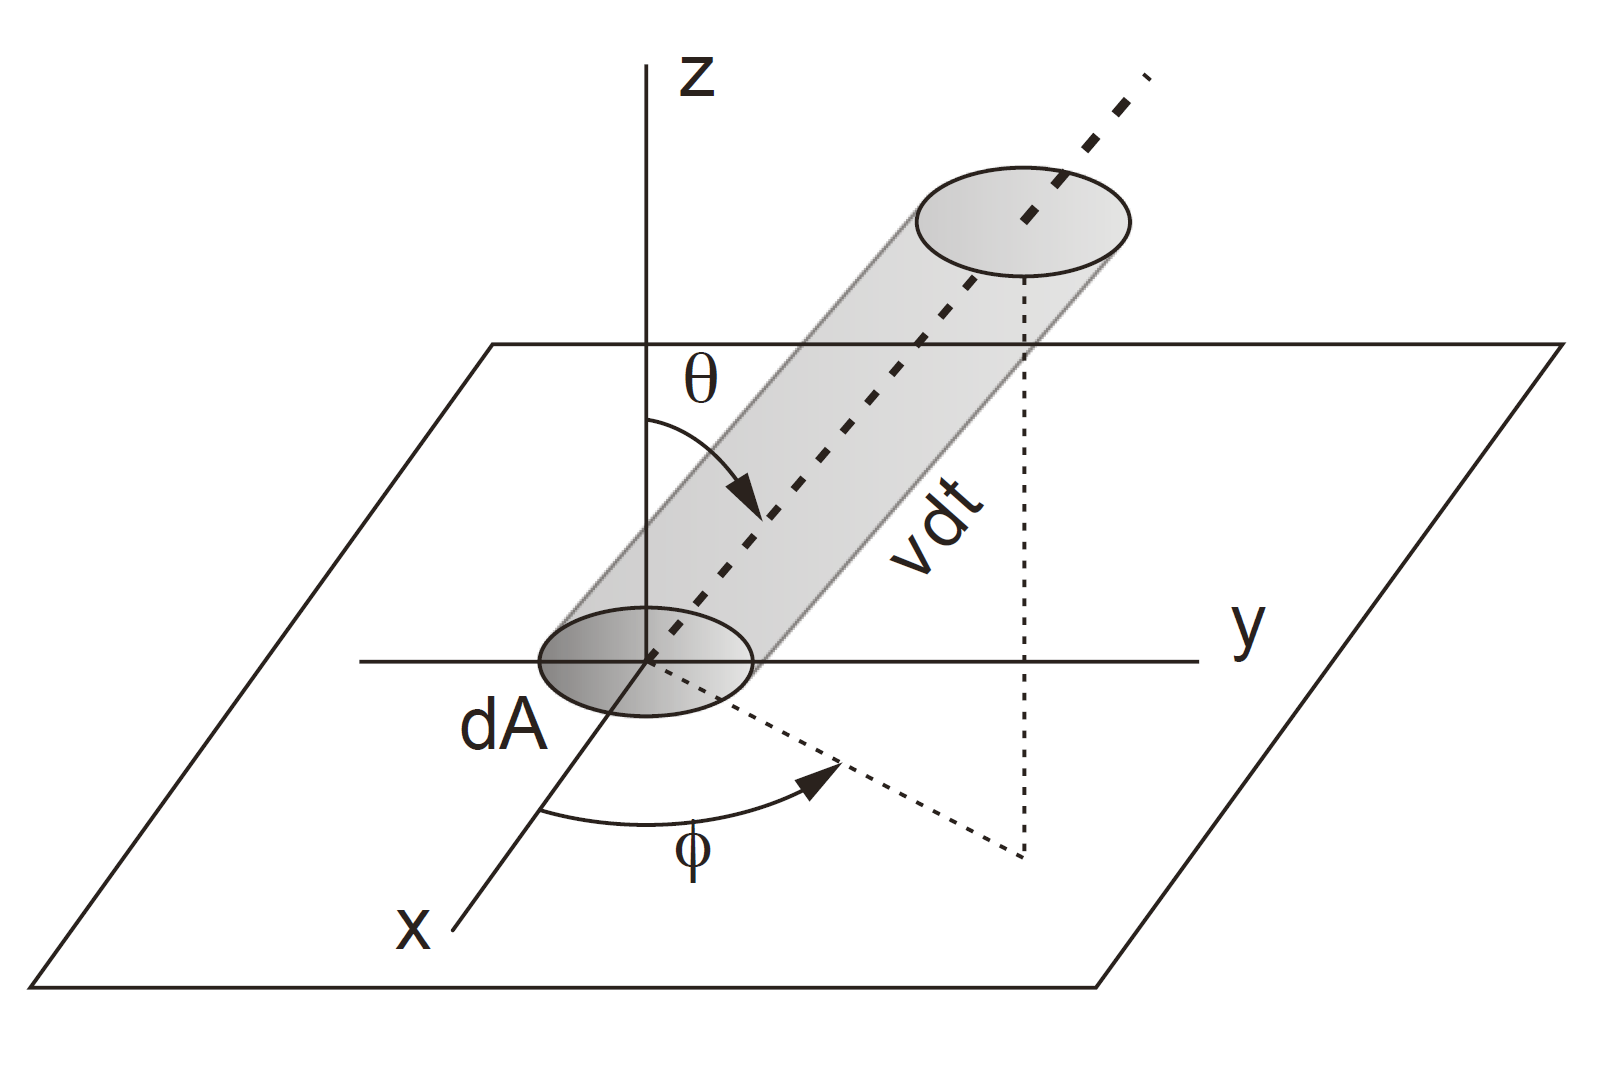
\includegraphics[width=0.30\textwidth]{cilindrooblicuo.png}
    \caption{cilindro oblicuo}
    \label{Fig:6.2-cilindro}
\end{wrapfigure}


En base a esto vamos a definir según la teoría cinética la presión. Primero vamos a estudiar cuanto cambia la cantidad de movimiento cuando una molécula choca, para luego estudiar cuantas moléculas chocan. Entonces la variación del momento de una partícula coincide con la variación de la cantidad de movimineto de la misma dirección normal a la pared. Entonces una partícula que choca con un ángulo $\theta$ respecto la normal (el momento tangencial se conserva) tenemos que el momento de salida menos el de entrada: 

\newpage

\begin{equation}
\Delta (m \cdot v) = m v \cos \theta - (- m v \cos \theta) = 2 m v \cos \theta
\end{equation}



Ahora el número de moléculas que chocan con la superficie $\D A$ (en este caso es unidad de superficie de la pared) con ángulo $\theta$  en un intervalo de tiempo $\D t$ es está contenido en un cilindro oblícuo \ref{Fig:6.2-cilindro} de base $\D A$. En esa unidad de tiempo solo las partículas que estén a una distancia menor o igual que $v \D t$ chocarán con la pared, por ello la longitud del cilindro será esta, y su altura será $ v \cos \theta \D t$. El volumen del cilindro:

\begin{equation}
\D V = v \cos \theta \D A  \D t
\end{equation} 

y por tanto el número de colisiones contra la superficie $\D A$ en un tiempo $\D t$ es de moléculas que lleven una velocidad $v$:

\begin{equation}
\D N_ {\theta, \phi, v}^{colisiones} = \D n_{\theta, \phi,v} \D V = \dfrac{\D n_v}{4 \pi} m v^2 \sin \theta  \cos \theta \ \D A \ \D \phi \ \D \theta \ \D t
\end{equation}

Entonces la variación de momento será el número de colisiones por la variación de momento por molécula:

\begin{equation}
\D (m \cdot v) = \dfrac{n_v}{2 \pi} m v^2 \sin \theta \cos^2 \theta\ \D A \ \D \phi \ \D \theta \ \D t
\end{equation}

y como $\D p = \dfrac{\D (m \cdot v)}{\D t \D A}$ (derivada del momento fuerza, fuerza por unidad de superficie presión):

\begin{equation}
\D p = \dfrac{n_v}{2 \pi} m v^2 \sin \theta \cos^2 \theta \ \D \phi \ \D \theta 
\end{equation}

La presión de total entonces vendrá dada por la suma de todas las velocidades en todos los cilindros posibles, por lo que habrá que integrar: $\theta \in (0,\pi/2), \phi \in (0, 2 \pi), v \in (0, \infty)$. Integramos entre 0 e infinito aunque está mal: realmente existe una velocidad superior (velocidad de la luz), y la velocidad $0$ es imposible de llegar (implica 0 K, violando el tercer principio de la termodinámica). Sin embargo son tan pocas las moléculas que tienen una velocidad extremadamente alta o extremadamente baja, integrar entre estos límites no supone un error. Entonces la presión vendrá dada por:

\begin{equation}
p = \dfrac{m}{2 \pi} \int_{0}^{\infty} v^2 \D n_v \int_{0}^{\pi/2} \sin \theta \cos^2 \theta \D \theta \int_0^{2 \pi} \D \phi = \dfrac{m}{3} \int_{0}^{\infty} v^2 \D n_v
\end{equation}\\



Ahora vamos a introducir unas definiciones importantes respecto las velocidades. Definimos como \textbf{vector velocidad media} como la media estadística de los vectores velocidad de las partículas en un instante dado:

\begin{equation}
\overline{\vec{v}}= \langle \vec{v} \rangle = \dfrac{V}{N} \into \vec{v} \D n_v
\end{equation}

el \textbf{valor medio de los cuadrados de las velocidades} como:

\begin{equation}
\overline{v^2} = \langle v^2 \rangle = \dfrac{V}{N} \into v^2 \D n_v
\end{equation}

y como \textbf{velocidad cuadrática media por:}

\begin{equation}
v_{cm} = \sqrt{ \langle v^2 \rangle}
\end{equation}

Entonces la presión se puede definir como:

\begin{equation}
p V = \dfrac{1}{3} m N \bar{v^2}
\end{equation}

\section{Consecuencias de la Ecuación cinética del gas perfecto}

Tenemos que el número de moles de un sistema es igual al número de partículas entre el número de avogadro. Entonces para un gas perfecto:

\begin{equation}
p V = n RT = \dfrac{N}{N_A} RT = N k_B T
\end{equation}

donde $k_B = R/N_A$ siendo esta la llamada \textbf{constante de Boltzmann}. Como sabemos que la presión depende de la velocidad cuadrática media, podemos relacionar la temperatura con la velocidad:

$$ \dfrac{1}{3} m N \overline{v^2} = N k_B T $$

en consecuencia:

\begin{equation}
\overline{v^2} = \dfrac{3 k_b T}{m} = \dfrac{3 R T}{M}
\end{equation}

Entonces está claro que: 

\begin{equation}
U = E_c = \dfrac{3}{2} N k_B T = \dfrac{3}{2} n RT
\end{equation}

De esto podemos deducir que: 

\begin{equation}
p = \dfrac{1}{3} \dfrac{N k_B T}{V} = \dfrac{2}{3} \dfrac{U}{V}
\end{equation}

Una vez hemos deducido la expresión de la energía interna del gas podemos deducir la expresión para el calor específico isocóro:

\begin{equation}
C_V = \pparciales{U}{T}_V = \dfrac{3}{2} n R
\end{equation}

\chapter{Funciones de distribución}

En este tema vamos a tratar de establecer cómo se encuentran distribuidas las velocidades de las moléculas del gas, y conocidas las distribuciones, como se encuentran distribuidos los diversos tipos de energía, estudiando finalmente el principio de equipartición de energía.

\section{Función de distribución de velocidades}

Recordemos los postulados con los que iniciábamos la teoría cinética:

\begin{itemize}
\item Isotropía de las velocidades: todas las direcciones de las velocidades son igualmente probables. No existe una dirección preferida/dispreferida.
\item La distribución de las velocidades es independiente del elemento de volumen que se considere independiente del tiempo.
\item El valor de una componente de la velocidad en un momento dado es independiente del valor de las otras componentes
\end{itemize}

Vamos a tratar ahora de determinar cuantas moléculas tienen una velocidad de dirección y magnitud especificada, lo que se conoce como \textit{ley de distribución de Maxwell}. \\


Supongamos que existe una función de distribución de velocidades $f(v_x)$ que nos de la probabilidad de encontrar una valor de la variable $v_x$ comprendido entre $v_x$ y $v_x + \D v_x$ para una componente particular, de tal modo que: 

\begin{equation}
\dfrac{\D N_{v_x}}{N} = f(v_x) \D v_x \label{ec:7.1-001}
\end{equation}

donde $N$ es el número total de particulas y pro lo tanto $\D N_{v_x} / N$ es la fracción de moléculas cuya velocidad está entre $v_x$ y $\D v_x$. Podemos hacer un procedimiento análogo para las otras componentes:

\begin{equation}
\dfrac{\D N_{v_y}}{N} = f(v_y) \D v_y
\end{equation}

\begin{equation}
\dfrac{\D N_{v_z}}{N} = f(v_z) \D v_z
\end{equation}

Por ser las velocidades independientes se puede deducir que:

\begin{equation}
\dfrac{\D N_{v_x, v_y, v_z}}{N} = \dfrac{\D N_v}{N} = f(v_x, v_y, v_z) \D v_x  \D v_y \D v_z = f(v)  \D v_x \D v_y \D v_z
\end{equation}
donde $  \D v_x \D v_y \D v_z$ es el \textit{elemento de volumen en el espacio velocidades}. No es trivial demostrar que:

\begin{equation}
f(v) = f(\sqrt{v_x^2 + v_y^2 + v_z^2}) = f(v_x) f(v_y) f(v_z) 
\end{equation}
Ahora vamos a relacionar las diferentes velocidades entre sí. Derivamos la ecuación anterior respecto $v_x$ (recordemos que $v= \sqrt{v_x^2 + v_y^2 + v_z^2}$):
$$
 \parciales{f(v)}{v_x} = \parciales{f(v)}{v} \parciales{v}{v_x} = \parciales{f(v)}{v} \dfrac{v_x}{v} = f(v_y) f(v_z) \parciales{f(v_x)}{v_x} \longrightarrow  
$$

\begin{equation}
\parciales{f(v)}{v} \dfrac{1}{v} =
\parciales{f(v_x)}{v_x} \dfrac{1}{v_x}
\end{equation}


De manera análoga


\begin{equation}
\parciales{f(v)}{v} \dfrac{1}{v} = 
\parciales{f(v_y)}{v_y} \dfrac{1}{v_y}
\end{equation}


\begin{equation}
\parciales{f(v)}{v} \dfrac{1}{v} = 
\parciales{f(v_z)}{v_z} \dfrac{1}{v_z}
\end{equation}

Es decir:

\begin{equation}
\parciales{f(v_x)}{v_x} \dfrac{1}{v_x} =
\parciales{f(v_y)}{v_y} \dfrac{1}{v_y}= 
\parciales{f(v_z)}{v_z} \dfrac{1}{v_z} = \mathrm{cte} = - 2B
\end{equation}

de tal forma que si integramos obtenemos que:

\begin{equation}
\logn f(v_x) = - B v_x^2 + \logn A \Longrightarrow f(v_x) = A e^{- B v_x^2}
\end{equation}

tanto $A$ como $B$ son positivas ya que de lo contrario la probabilidad sería negativa y para altas velocidades en $v \rightarrow \infty$ serían muy probables. Substituímos esto en la ecuación \ref{ec:7.1-001}, obteniendo la \textbf{ley de distribución de velocidades vectoriales para la componente x}:

\begin{equation}
\dfrac{\D N_{v_x}}{N} = A e^{-Bv_x^2} \D v_x  \label{ec:7.1-011}
\end{equation}

y para la general, dando la llamad \textbf{ley de Maxwell de la distribución de velocidades vectoriales}:


\begin{equation}
\dfrac{\D N_{v}}{N} = A^3 e^{-Bv^2} \D v_x \D v_y \D v_z
\end{equation}

Para que la integral de la función de probabilidad en todas las velocidades posibles sea uno, se tiene que verificar que:

\begin{equation}
A = \sqrt{\dfrac{B}{\pi}} \label{ec:7.1-013}
\end{equation}

Si en vez de integrar la velocidad en los componentes de la misma (espacio de velocidades cartesianos) integramos en el espacio de velocidades esféricas, por lo que aparecerá el módulo de la velocidad. Entonces tenemos que:

\begin{equation}
\dfrac{\D N_{v}}{N} = A^3 e^{-Bv^2} \D v_x \D v_y \D v_z = A^3 e^{-Bv^2} 4 \pi v^2 \sin \theta \ \D v \D \theta \D \phi 
\end{equation}

por lo que integrando en $\phi$ y $\theta$ (y usando ya la ecuación \ref{ec:7.1-013}) obtenemos que:

\begin{equation}
f(v) = \parentesis{\dfrac{B}{\pi}}^{3/2} 4 \pi v^2 e^{-B v^2}
\end{equation}


de tal modo que obtenemos la \textbf{ley de distribución de las velocidades escalares}:

\begin{equation}
\dfrac{\D N_v}{N} = \parentesis{\dfrac{B}{\pi}}^{3/2} 4 \pi v^2 e^{-Bv^2} \D v \label{ec:7.1-016}
\end{equation}

Calculemos ahora la \textit{media de los cuadrados de la velocidad}, que viene dada por: 

$$ \overline{v^2} = \into v^2 \D N_v  = 4 \pi \parentesis{\dfrac{B}{\pi}}^{3/2} \into v^4 e^{-Bv^2} \D v = 4 \pi \parentesis{\dfrac{B}{\pi}}^{3/2} \dfrac{3}{8} \parentesis{\dfrac{\pi}{B^5}}^{1/2} \Longrightarrow $$

\begin{equation}
B = \dfrac{3}{2} \dfrac{1}{\overline{v^2}} = \dfrac{m}{2 k_B T}
\end{equation}

En la figura se pueden ver las distribuciones de velocidades escalares para distintas temperaturas. A mayor temperatura mayores velocidades, y la función se ensancha, siendo las velocidades mas probables cada vez mayores pero decreciendo en cuanto a frecuencia. El efecto de la masa es al revés, a mayor masa la función se estrecha y es mas probable encontrar velocidades cada vez mas pequeñas. Usando las definiciones del tema anterior:

\begin{itemize}
\item \textbf{Velocidad mas probable} $v_m$: 

\begin{equation}
v_m = \sqrt{\dfrac{2 k_B T}{m}}  = \sqrt{\dfrac{1}{B}}
\end{equation}

\item \textbf{Velocidad cuadrática media} $v_{cm}$:

\begin{equation}
v_{cm} = \sqrt{\dfrac{3 k_B T}{m}} = \sqrt{\dfrac{3}{2B}}
\end{equation}

\item \textbf{Velocidad media} $\bar{v}$:

\begin{equation}
\bar{v} =  \sqrt{\dfrac{8 k_B T}{\pi m}} = \sqrt{\dfrac{4}{\pi B}} 
\end{equation}
\end{itemize}

donde se puede ver claramente que $v_{cm} > \bar{v} > v_,m$. En los ejercicios muchas veces nos encontraremos que nos piden que calculemos el número de moléculas que hay (respecto el total, o las totales) entre dos velocidades. A veces nos la dan para una componente la velocidad o para el módulo. En el caso de que sea de la primera debemos integrar la ecuación \ref{ec:7.1-011}, para lo cual es interesante usar la \textbf{función error} $F_{err} (x)$ tabulada:

\begin{equation}
F_{err} (x) = \dfrac{2}{\pi} \int_0^x e^{-x^2} \D x
\end{equation}

\section{Función de distribución de energías}

Sabemos que la energía de una partícula viene dada por:

$$ E = \dfrac{1}{2} m v^2 \Longrightarrow \D E = m v \D v \Longrightarrow \D E = \sqrt{2 m E} \D v $$

si substituimos la energía por la velocidad y sus diferenciales en la ecuación \ref{ec:7.1-016} podemos obtener que:

\begin{equation}
\dfrac{\D N_E}{N} = \dfrac{2}{\sqrt{\pi}} (k_B T)^{-3/2} \sqrt{E} e^{-E/k_B T} \D E
\end{equation}

a esta última ecuación la llamamos \textbf{ley de distribución de la energía de traslación}, y nos dice el número de moléculas cuya energía de traslación está comprendida entre $E$ y $E + \D E$. Solo es función de la temperatura, sin importar el gas. La \textbf{energía mas probable} vendrá dada por:

\begin{equation}
E_m = \dfrac{1}{2} k_B T
\end{equation}

Y la energía correspondiente a la velocidad mas probable es:

\begin{equation}
E_{v_m} = 2 E_m = k_B T
\end{equation}

en donde la \textbf{energía de traslación media molecular } $\bar{E}$ viene dada por:

\begin{equation}
\overline{E} = \dfrac{1}{N} \into E \D N_E  = \dfrac{3}{2} k_B T
\end{equation}

\section{Principio de equipartición de energía}

Podremos calcular cual es la energía asociada a una determinada componente de la velocidad de tal forma que:

\begin{equation}
\overline{E_x} = \dfrac{1}{2} m \overline{v^2_x}
\end{equation}

Si integramos entre (-$\infty, \infty$) la velocidad $v_x$ (puede tener sentido positivo o negativo la velocidad), obtenemos que:

\begin{equation}
\overline{v^2_x} = \dfrac{1}{2 B} = \dfrac{k_B T}{m}
\end{equation}

Como $y$ y $z$ son independientes estas valdrán lo mismo que $\overline{E_x}$, que además serán un tercio de energía de traslación media:

\begin{equation}
\overline{E_x} = 
\overline{E_y} =
\overline{E_z} = \dfrac{1}{3} \overline{E}
\end{equation}

En nuestro modelo del gas ideal las moléculas monoatómicas presentan tres modos de movimiento independientes entre sí, correspondientes a los movimientos en cada una de las direcciones espaciales. Cada uno de estos modos contribuye $(1/2) k_B T$ a la energía de la molécula. Como la energía cinética traslacional está igualmente dividida para cada uno de los modos decimos que existe una \textit{equipartición} de energía. Llamamos \textit{grado de libertad} a cada una de las variables independientes necesarias para especificar la energía de una molécula. \\

Si por ejemplo una molécula puede girar sobre si misma tenemos que añadir su energía de rotación, o si tiene varios átomos girar entorno a sus ejes principales (varias energías de rotación). Incluso las distancias entre los átomos pueden variar (vibración) por lo que habría que añadir esta energía. \\
 
Si una molécula posee $f$ grados de libertad y la energía asociada a cada grado de libertad es de una forma cuadrática, el valor medio de la energía correspondiente a cada uno de dichos grados de libertad es $(1/2)k_B T$, lo que se conoce como \textbf{principio de equiparticipación de la energía}, tal que:

\begin{equation}
\overline{E} = \frac{f}{2} k_B T
\end{equation}

Si no existen campos externos y una energía cinética macroscópica (el sistema no se desplaza), la energía cinética interna del sistema se identifica con la energía cinética de las partículas del gas. Obviamente las moléculas poseen energías rotacionales, vibracionales, incluso electrónicas, pero dado que estas últimas tienen ordenes mucho menores a la energía traslacional y las moléculas monoatómicas no tienen rotaciones ni vibraciones, es por lo que identificamos la energía de una molécula monoatómica por la suma de energías cinéticas. Para una molécula con $f$ grados de libertad:

\begin{equation}
U = N \overline{E} = \dfrac{f}{2} n RT
\end{equation}

y por lo tanto para el gas ideal:

\begin{equation}
c_V = \dfrac{\D U}{\D T} = \dfrac{f}{2} R
\end{equation}

expresión que relaciona la capacidad calorífica molar con los grados de libertad de las moléculas, y se conoce como \textit{teoría clásica de los calores específicas}.

\section{Aplicaciones ley de distribución}

Si tenemos en cuanta que el número de moléculas con velocidades comprendidas entre $v$ y $v + \D v$ que chocan contra una superficie por unidad de área y unidad de tiempo, formando ángulos comprendidos en los intervalos $\theta$ y  $\theta + \D \theta$; $\phi$ y $\phi + \D \phi$ viene dado por:


\begin{equation}
\dfrac{\D N^{col}_{v,\theta,\phi}}{\D A \D t} = \dfrac{v \D n_V}{4 \pi} \sin \theta \D \theta \D \phi
\end{equation} 

donde llamamos al número de choques por unidad de área y tiempo como \textbf{frecuencia de colisión}, para cualquier velocidad y dirección, al término que surge de integrar las velocidades, y los ángulos, tal que:

\begin{equation}
\dfrac{\D N^{col}_{v,\theta,\phi}}{\D A \D t} = \dfrac{n \bar{v}}{4}
\end{equation}

Si en lugar de una superficie existiese un pequeño orificio en al pared del recipiente que contiene al gas la expresión anterior nos daría el número de moléculas por unidad de tiempo y área que se escapan por dicho orificio, que notaremos por $n_e$. A este fenómeno lo conocemos por \textbf{efusión}. 

\begin{equation}
n_e = \dfrac{\D N^{esc}}{\D A \D t } = - \dfrac{N}{V} \sqrt{\dfrac{RT}{2 \pi M}}
\end{equation}

también podemos indicar que $n_e = J_n$ ya que no es mas que el flujo de partículas a través del orificio por unidad de superficie y tiempo. \\

Es muy importante que el orificio sea lo suficientemente pequeño como para que se escapen pocas moléculas y se mantenga la distribución de velocidades en equilibrio, además de mantener así la presión constante y evitar que se produzcan flujos macroscópicos de gas. Otra condición es que las paredes del recipiente deben ser delgadas para reducir en la medida de lo posible las colisiones con los cantos del orificio (esto produciría re-entradas de las moléculas). \\

En la práctica crear estos orificios es muy complicado.  Sin embargo la efusión tiene muchas propiedades prácticas, como la separación de isótopos de determinados elementos ya que el número de moléculas es inversamente proporcional a la masa molar, la determinación de presiones de vapor de líquidos y sólidos... 

\chapter{Fenómenos de transporte}

Llamamos \textbf{fenómenos de transporte} a aquellos procesos físicos en los que tiene lugar un flujo de alguna magnitud física (masa, carga, energía, cantidad de movimiento...) en respuesta a una distribución no uniforme de la misma. Empíricamente se sabe que las causas de este transporte se deben a que el número de partículas por unidad de volumen que poseen un valor determinado de la propiedad no es uniforme, y por tanto a escala microscópica estos fenómenos se le atribuye al transporte molecular de las magnitudes físicas. \\
 
Entonces cuando la concentración de partículas varía se origina una \textit{difusión}, cuando el número de partículas por unidad de volumen poseen una energía cinética que varía se produce una \textit{conducción térmica}, y si consideramos la cantidad de movimiento como magnitud transportada explicaremos la \textit{viscosidad}, y la \textit{conducción eléctrica} si varía la carga eléctrica por unidad de volumen. \\

Dado que los fenómenos de transporte se producen por el gradiente de alguna magnitud física, el sistema no se encontrará en equilibrio termodinámico, aunque su estado pueda ser estacionario. Todos estos fenómenos dependen de las colisiones de las partículas del sistema. En consecuencia para el estudio de los fenómenos de transporte se necesitarán conocer la distribución molecular en función de la posición y tiempo. \\

En este capítulo vamos a usar un método simplificado, para el que tendremos que imponer condiciones. Las primeras condiciones serán las hipótesis que hemos usado para desarrollar la teoría cinética. Además el tratamiento no será válido para presiones altas (ya que las fuerzas intermoleculares a presiones altas tienen una gran importancia) ni bajas (es mas probable chocar con la pared que con otra molécula). Otra condición es que el recorrido libre medio debe ser mayor que el diámetro molecular y menor que las dimensiones del recipiente. 

\section{Frecuencia de colisión}

En el desarrollo de la teoría cinética del gas ideal hemos supuesto que las moléculas son esferas rígidas que sufren colisiones perfectamente elásticas entre sí y prácticamente instantáneas (no existen interacciones intermoleculares). \\

En ausencia de campos externos las moléculas entre colisión y colisión se moverán en línea recta, por lo que la molécula acaba describiendo un recorrido en zig-zag. \\

Supongamos un sistema con dos tipos de moléculas, una de diámetro $d_1$ y masa $m_1$, y la otra de diámetro $d_2$ y masa $m_2$, moviéndose a velocidades $\bar{v_1}$ y $\bar{v}_2$, habiendo en la mezcla un número de moléculas $N_1$ y $N_2$. El número de moléculas por unidad de volumen se denotará por $n_1$ y $n_2$. \\

Para que se produzca una colisión los centros de las moléculas deben estar separados por una distancia $d$ menor o igual a la suma de ambos radios, que denominaremos por $d$ tal que:

\begin{equation}
d = \dfrac{d_1 + d_2}{2}
\end{equation}

a este parámetro lo llamamos \textbf{diámetro de colisión} o \textbf{diámetro efectivo}. Llamamos \textbf{sección eficaz} al área de la circunferencia formada por un círculo de radio $d$. Viene a representar el área en el cual se debe de encontrar el centro de una molécula 1 para que colisione con la molécula 2. Si el centro se encuentra en esta superficie habrá colisión, si no, no la habrá. Denotamos por $\sigma$ a la sección eficaz:

\begin{equation}
\sigma = \pi d^2
\end{equation}

Supongamos ahora que la molécula 2 está quieta y es la molécula 1 la que se mueve a una velocidad relativa media de $\bar{v}_12$. La molécula en un tiempo $\D t$ barrerá un volumen cilíndrico $$ \sigma \bar{v_{12}} \D t $$ tal que si hay una molécula de tipo 2 cuyo centro este dentro de este volumen habrá una colisión. El número de moléculas de tipo 2 que habrá dentro del cilindró vendrá dada por:

$$ n_2 \sigma \bar{v_{12}} \D t $$

que será el número de colisiones que sufre la molécula de tipo 1 con la de tipo 2 en dicho intervalo de tiempo. Por lo tanto la frecuencia (choques por unidad de tiempo) vendrá dada por:

\begin{equation}
Z_1 (2) = n_2 \sigma \bar{v_{12}}
\end{equation}

siendo esta la \textbf{frecuencia de colisiones}. La velocidad relativa media se puede obtener fácilmente usando la expresión:

\begin{equation}
(\bar{v}_{12})^2 = (\bar{v}_1)^2 + (\bar{v}_2)^2
\end{equation}

que al ser un sistema con la misma temperatura $T$ se pueden expresar la suma de las velocidades como:

\begin{equation}
(\bar{v}_{12})^2 = \dfrac{8 k_b T}{\pi} \parentesis{\frac{1}{m_1} + \frac{1}{m_2}} = \dfrac{8 k_b T}{\pi \mu} 
\end{equation}

Si lo llevamos a la frecuencia de colisión entre las dos moléculas:

\begin{equation}
Z_1 (2) = n_2 \sigma \sqrt{\frac{8 k_B T}{\pi \mu}}
\end{equation}

y si queremos saber la frecuencia total de colisiones tipo 1-2 tenemos que multiplicar la frecuencia con la que choca una partícula de tipo 1 con una de tipo 2 por el número de moléculas de tipo 1. Entonces:

\begin{equation}
Z_{12} = N_1 \sigma n_2  \sqrt{\frac{8 k_B T}{\pi \mu}}
\end{equation}

o por unidad de volumen:

\begin{equation}
z_{12} = \sigma n_1 n_2  \sqrt{\frac{8 k_B T}{\pi \mu}}
\end{equation}

Podemos calcular de manera completamente análoga la frecuencia de colisión entre moléculas de tipo 1 con otras de tipo 1 y de tipo 2 con otras de tipo 2. La frecuencia con la que choque una partícula con otra será la suma de la frecuencia de que choque contra partículas de otro tipo y contra partículas de su mismo tipo. \\

Recordemos que este método es particularmente limitado: no solo tenemos las limitaciones de la teoría cinética, además hemos considerado que solo hay colisiones binarias. Aunque en general esto no supondrá un problema si estamos ante un gas a baja densidad. 

\section{Recorrido libre medio}

Se conoce como \textbf{recorrido libre medio} $\lambda$ a la distancia media recorrida por una molécula de un gas entre dos colisiones sucesivas. Aunque la distancia no es constante, si que lo es su recorrido libre medio. Dado que la frecuencia de colisión es $Z$, tenemos que el tiempo que tarda en colisionar será la inversa de la frecuencia. Si a este tiempo lo multiplicamos por la velocidad media hallaremos el recorrido libre medio:

\begin{equation}
\lambda = \frac{\bar{v}}{Z} =  \frac{1}{\sqrt{2} n \sigma} = \frac{k_B T}{\sqrt{2} \sigma p}
\end{equation}

donde la última igualdad se hace teniendo en cuenta la ecuación para un gas ideal $N/V = p/k_BT$. Si nuestro gas resulta ser una mezcla de dos diferentes tipos de moléculas el recorrido libre medio cambiará: 

\begin{equation}
\lambda_1 = \dfrac{\bar{v_1}}{Z_1(1) + Z_1(2)} \tquad 
\lambda_2 = \dfrac{\bar{v_2}}{Z_2(1) + Z_2(2)}
\end{equation}

donde $Z_i(j)$ representa la frecuencia de que una partícula $i$ colisione con una de tipo $j$. \\

Procederemos ahora a estudiar la \textit{ley de distribución de recorridos libres}. Esta nos dará una medida de que fracción de moléculas recorren \textit{sin colisionar} con otras una longitud comprendida entre $r$ y $r + \D r$ después de haber realizado una colisión. Sea $N_0$ el número inicial de moléculas y $N$ el número de moléculas de dicho grupo que no ha efectuado ninguna colisión en una distancia $r$ medida a lo largo del recorrido libre de cada molécula, se tiene que verificar que en el siguiente tramo $\D r$ cierto número de moléculas chocarán y $N$ se reducirá, por lo que;

\begin{equation}
\D N = - \alpha N \D r
\end{equation}

siendo $\alpha$ un coeficiente de proporcionalidad. Si integramos deducimos que:

\begin{equation}
N = N_0 e^{-\alpha r}
\end{equation}

por la definición del recorrido libre medio:

\begin{equation}
\lambda = \bar{r} = \dfrac{\into r \D N}{\into \D N} = \dfrac{1}{\alpha}
\end{equation}

por lo que la \textbf{ley de distribución de recorridos libres} también llamada \textbf{ecuación de supervivencia} tenemos que:

\begin{equation}
N = N_0 e^{-r/\lambda} \tquad \D N = - \dfrac{N_0}{\lambda} e^{-r / \lambda} \D r
\end{equation}

De manera exactamente análoga podemos calcular cual es el valor medio de la distancia a un elemento de superficie a la cual una molécula realiza su última colisión antes de alcanzar dicha superficie y cruzarla si fuese imaginaria. Podemos deducir con facilidad qeu el número total de partículas que alcanzan dicho elemento de superficie $\D A$ desde cualquier dirección y distancia vendrá dada por:

\begin{equation}
\D N^{colis} = \dfrac{1}{4} n \lambda Z \D A \D t = \dfrac{1}{4} \bar{v} n \D A \D t
\end{equation}

\section{Transporte de cantidad de movimiento: viscosidad}

Aplicando nuestro conocimiento sobre el recorrido libre medio analizaremos como se transporta la cantidad de movimiento, que nos permite definir la viscosidad de un gas. De manera sencilla podemos definir viscosidad como la resistencia al flujo que oponen los fluidos. No es mas que una constatación de la existencia del rozamiento interno cuando los fluidos se encuentran en movimiento. \\

Para llevar acabo un análisis sencillo diremos que las moléculas son esferas rígidas y sin fuerzas intermoleculares, de masa $m$, diámetro $d$ y concentración $n$. Si consideramos que el fluido se encuentra confinado entre dos placas paralelas entre sí, separadas por una dis tancia pequeña $h$. Ahora tratamos de empujar ahora una de las placas (la placa superior) con una fuerza (la de abajo está fija) constante. Lo que ocurrirá una vez llegado el estado estacionario es que para cada altura $z$ el fluido tendrá una velocidad diferente en el eje x (la fuerza se ejerce en dirección x). Entonces habrá un gradiente de velocidades no nulo en función de la altura.\\

Se verificará ademas que para la altura 0 (justo encima de la placa fija) la velocidad es 0 ($v(0)=0$), y que para la altura $h$ la velocidad será $v_p$ ($v(h)=v_p$). Podemos imaginarnos esto laminando el fluido. Imaginemos que el fluido está subdividido en muchas capas delgadas (láminas) paralelas a los dos planos. Como consecuencia del rozamiento interno la capa superior arrastrará a la capa inferior. De etsa forma la capa de arriba cede parte de su cantidad de movimiento a la mas lenta, por lo que hay una transferencia de cantidad de movimiento en la dirección del eje y (altura). \\

La \textit{ley de Newton de la viscosidad} nos dice como se relacionan fuerza, área, viscosidad y velocidad en función de la altura. Esta es:

\begin{equation}
\dfrac{F_x}{A} = \eta \dfrac{\D v_x}{\D y} = \tau_{yx}
\end{equation}

donde $\eta$ es el \textbf{coeficiente de viscosidad absoluta} definido positivo. El parámetro $\tau_{yx}$ es la tensión de corte, cizalla o fuerza cortante por unidad de superficie, siendo y el vector normal superficie y x la dirección de la fuerza. Como podemos ver la tensión cortante tiene unidades de cantidad de movimiento por unidad de área y tiempo, es decir, representa un  \textbf{flujo de cantidad de movimiento}:

\begin{equation}
\Jn_p = - \eta \dfrac{\D v_x}{\D y} \mathbf{j}
\end{equation}

donde el signo negativo indica simplemente que el sentido del flujo es opuesto al gradiente de la velocidad. Podemos deducir que la viscosidad viene dada por:

\begin{equation}
\eta = \dfrac{1}{3} m \bar{v} n \lambda = \dfrac{1}{3 \sqrt{2}} \dfrac{m \bar{v}}{\sigma} = \dfrac{1}{3 \sqrt{2}} \dfrac{m}{\sigma} \sqrt{\dfrac{8 k_B T}{\pi m}} = \dfrac{2}{3 \sqrt{\pi}} \dfrac{\sqrt{MRT}}{N_A \sigma}
\end{equation}

\section{Transporte de energía. Conductividad térmica}

La \textbf{conducción térmica} en un gas se pone de manifiesto cuando existe una diferencia de temperatura entre distintas regiones de la masa gaseosa, lo que provoca un flujo térmico desde las regiones de mayor temperatura a las de menor temperatura. \\

Como no existe desplazamiento global de materia ni variación macroscópica de la energía del sistema, ni se pone en juego trabajo mecánico decimos que este flujo térmico es un flujo \textit{no convectivo} de la energía interna del gas. El análisis de este tipo de transporte nos va a permitir dar una justificación molecular del \textbf{coeficiente de conductividad térmica}. 

\section{Transporte de masa. Difusión}


\end{document}


